% File: main.tex: TMLR camera-ready (single column).
% Sections are shared with paper/sections/; the appendix is merged after the
% references, as TMLR requires (paper_tmlr/appendix_body.tex is generated from
% paper/appendix.tex by scripts/revision_generate_appendix.py).
\documentclass[10pt]{article}
\usepackage[accepted]{tmlr}

% hidelinks: keep cross-references clickable without hyperref's default
% coloured boxes, which the TMLR template leaves on and which print badly.
\usepackage[hidelinks]{hyperref}
\usepackage{url}

% Math + theorem environments.
\usepackage{amsmath}
\usepackage{amssymb}
\usepackage{amsthm}
% GENERATED from revision_results/statistics.json.
\newcommand{\RevEOneMean}{0.1245}
\newcommand{\RevEOneTLow}{-0.0406}
\newcommand{\RevEOneTHigh}{0.2896}
\newcommand{\RevEOneBLow}{-0.0180}
\newcommand{\RevEOneBHigh}{0.2830}
\newcommand{\RevEOneR}{0.4386}
\newcommand{\RevHarvest}{4.0107}
\newcommand{\RevPrediction}{4.1203}
\newcommand{\RevCorrectedPrediction}{4.3301}

\newtheorem{proposition}{Proposition}
\newtheorem{corollary}{Corollary}
\newtheorem{lemma}{Lemma}
% Unnumbered twins: the appendix restates body statements before proving them,
% so those restatements must not consume a number or a label.
\newtheorem*{propositionx}{Proposition}
\newtheorem*{corollaryx}{Corollary}
\theoremstyle{remark}
\newtheorem*{remarkx}{Remark}

\usepackage{booktabs}
\usepackage{graphicx}
% The appendix's small plots are 3.3in wide in a 6.5in column, so each one used
% to claim a whole row. subcaption lets the generator pair them two-up; see the
% pairing step in tools/make_tmlr_appendix.py.
\usepackage{subcaption}
% A paired float shares one figure number, so a pointer renders "Figure 10a"
% while stock subcaption prints only "(a)" on the panel: the number the reader
% was sent to find appears nowhere on the page. Print the full "Figure Na"
% instead. This swaps one label prefix for another, so unlike a parent caption
% or a per-panel \caption (both measured at +2 pages) it costs no space.
\DeclareCaptionLabelFormat{panel}{Figure \thefigure#2}
\captionsetup[subfigure]{labelformat=panel,labelsep=colon}
\usepackage{array}
\usepackage{microtype}

% Exact code identifiers (file:line citations) in the appendix audit registers.
% (TMLR's wider 10pt font also forces the audit tables' verdict columns to be
% rebalanced; that happens in the appendix generator, not here.)
\newcommand{\code}[1]{\texttt{#1}}
\newcolumntype{L}[1]{>{\raggedright\arraybackslash}p{#1}}

% Width of a "column" figure in this single-column layout. The shared section
% sources use \figwidthcol so one copy serves both venue builds; 0.62\textwidth
% keeps a figure drawn at 3.3125in from being blown up across the full 6.5in
% measure (Phase B re-renders these at native single-column size).
\newcommand{\figwidthcol}{0.62\textwidth}

% The harvest figure is the exception: its two panels are rendered side by
% side at exactly 6.5in, the full measure, so it is placed at native size.
% Stacked and scaled to \figwidthcol it stood 4.6in tall and was the tallest
% object in the body; two-up it is 2.6in and is not upscaled, which also means
% its 8pt floor is the size that actually reaches the page.
\newcommand{\figwidthharvest}{\textwidth}

% Diagnosis II is supplement-scoped. It is a correct result and it explains why
% the two diagnoses land on the same method family, but its evidence base
% (analytical plus three instrumented systems) is a different kind of thing
% from the audit that carries the paper, and stating it in the body invited
% reviewers to read the submission as two loosely-coupled papers. It therefore
% lives in the appendix, with one contribution sentence and a pointer here.
\newcommand{\diagtwoscope}{, supplement-scoped}
\newcommand{\diagtwopointer}{Appendix~\ref{sec:deadmeta-taxonomy} gives the
statement, the three escapes, and a per-system taxonomy, with the proof in
Appendix~\ref{sec:proofs}}
\newcommand{\contribdiagtwo}{(3) A second, supplement-scoped diagnosis
(Appendix~\ref{sec:deadmeta-taxonomy}) explains why this method family is the
one the audit keeps landing on: the canonical lr-scaled virtual step emits an
exactly $\eta$-scaled meta-signal (Proposition~\ref{prop:deadmeta}), which is
potentially dominated where an $\eta$-independent term of comparable or larger size competes
for the same weights. It is a magnitude ratio rather than a certainty, three
named escapes mitigate it, and we hold it to a lower evidentiary bar than the
rest of the paper: analytical, instrumented in three systems, not audited at
scale.}
% The two harvest-evidence floats. Declared as a macro so the shared
% section file can place them where Proposition 2 is discussed rather
% than at the top of the paper, which put both on page 3 five pages
% ahead of the statement they qualify. AAAI defines this empty.
% Two-up, not stacked. These are one piece of evidence about how far
% Proposition 2 transports: how badly the law misses a held-out seed, and how
% wide the intervals around its ratios really are. Standing them side by side
% halves the vertical footprint and stops the pair reading as two unrelated
% results. Both scripts render at 3.05in so the panels arrive at their typeset
% width instead of being scaled; 0.48 + 0.48 with \hfill cannot overlap.
\newcommand{\evidencefloats}{%
\begin{figure}[t]
\centering
\begin{subfigure}[t]{0.48\textwidth}
\centering
\IfFileExists{figs/fig_r1_crossseed.pdf}{%
  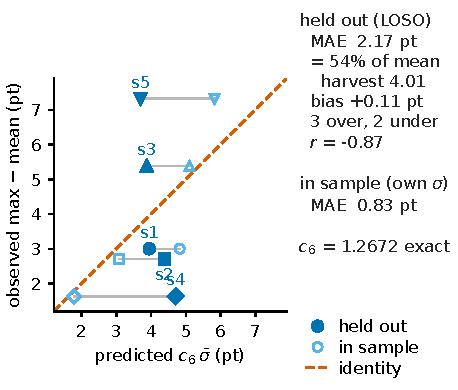
\includegraphics[width=\linewidth]{figs/fig_r1_crossseed.pdf}%
}{}
\caption{The preregistered leave-one-seed-out predictive check.
Estimating $\bar\sigma$ from four seeds and predicting the fifth's
max-minus-mean gives a mean absolute error of $2.17$ points ($54\%$ of the
$4.01$ being predicted), and the two series \emph{anti}-correlate
($r=-0.87$). This observed anticorrelation is not forced by leave-one-out
construction alone. Mean signed error is $+0.11$; substituting each seed's
own fitted $\sigma$ reduces MAE to $0.83$ but reuses the outcomes and is
not predictive validation. Neither the Gaussian shape nor transport of its
scale is established by this comparison.}
\label{fig:crossseed}
\end{subfigure}
\hfill
\begin{subfigure}[t]{0.48\textwidth}
\centering
\IfFileExists{figs/fig_r2_ratios_ci.pdf}{%
  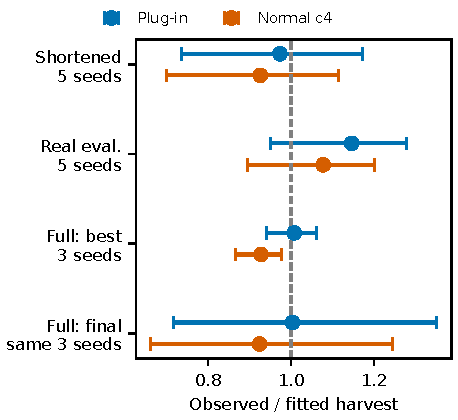
\includegraphics[width=\linewidth]{figs/fig_r2_ratios_ci.pdf}%
}{}
\caption{Same-sample harvest-to-scale ratios with joint whole-seed percentile
$95\%$ intervals, exhaustively enumerating the $n^n$ ordered resamples and
refitting the scale in each. Both plug-in and conditional Gaussian $c_4$
corrections are shown. The corrected full-protocol best-checkpoint interval
$[0.8665,0.9776]$ excludes one, but has only $27$ resamples from three seeds;
it is not reliable evidence against the model. Best and final use the same
three seeds, not independent replications.}
\label{fig:ratios}
\end{subfigure}
\end{figure}%
}
\newcommand{\evidencefigs}{ (Figures~\ref{fig:crossseed} and~\ref{fig:ratios};
the verification split is Figure~\ref{fig:ledger})}

% A forced \newpage used to live here, to hand the page carrying the two-up
% evidence float the three orphaned lines that preceded it. Re-rendering the
% harvest figure two-up (6.5 x 2.6in instead of 3.3125 x 3.80in scaled to
% 4.6in tall) freed about two inches on that page and made the break not just
% unnecessary but harmful: it pinned the freed space at the foot of page 7
% instead of letting it propagate. Removing it pulled the References onto
% page 12. \raggedbottom, set above, is what actually closes the float-to-text
% holes; the break never contributed to that.

% Let TeX stretch interword spacing rather than protrude into the margin: the
% appendix prose carries long unbreakable code identifiers.
\emergencystretch=1.5em

% The audit and registry tables are near-page-sized, and the supplement is
% figure-dense: let floats fill tops AND bottoms and share pages with text
% rather than each claiming a page, which is what keeps the merged document
% inside its length target.
\renewcommand{\topfraction}{0.92}
\renewcommand{\bottomfraction}{0.6}
\renewcommand{\textfraction}{0.05}
% 0.85, and it is still load-bearing after the CaffeNet figure (the float this
% was originally tuned for) was removed. Re-measured on the current document:
% 0.85 gives 38 pages with 6 underfull vboxes; 0.7 gives 39 with 2; deleting
% the line entirely gives 39 with 4. A lower threshold lets some float qualify
% for a page of its own instead of sharing one with text. The tallest float
% left is 0.44 of a text page, so nothing here is being forced. Re-measure
% before changing: the useful value depends on which floats exist.
\renewcommand{\floatpagefraction}{0.85}

% A page whose only content is a float (e.g. Table 2, page 17) was landing
% vertically CENTERED rather than pinned to the top. Cause, confirmed by
% testing: \flushbottom/\raggedbottom control the stretch around the whole
% text column and had zero effect (tested both); the actual glue is the
% kernel's float-page-only registers \@fptop / \@fpbot, which split the page's
% leftover height before and after the float. Both default to "0pt plus 1fil"
% (set in size10.clo, the 10pt option file, not in article.cls itself), so the
% two infinite stretches share the slack equally and centre the float. Zeroing
% \@fptop moves all of it to \@fpbot, the conventional "pinned to top" layout.
\makeatletter
\setlength{\@fptop}{0pt}
\makeatother

% tmlr.sty line 64 sets \flushbottom, and \parskip (line 169) is rigid, so on
% a page carrying a tall float there is almost no stretchable glue: TeX reaches
% \textheight by stretching \textfloatsep far past its 2pt "plus", opening a
% hole between the float and the text. That is what the log's Underfull \vbox
% entries were. Measured across the whole document: \flushbottom gave 7 such
% pages with a worst float-to-text hole of 55pt; \raggedbottom gives 0 and a
% worst of 23pt, at the same 35 pages and still 0 overfull hboxes. Ragged
% bottom parks the leftover at the foot of the page, where a slightly short
% page is ordinary, instead of wedging it above a paragraph. This overrides a
% tmlr.sty setting, but it touches only where slack sits, not the margins,
% font size, or leading, so it is not a format deviation.
\raggedbottom

% "Can Enable Selection Bias", not "Manufacture Gains". The probe does not
% manufacture anything on its own: it destroys a coupling, and a selection step
% that reads the affected quantity turns that into a one-sided gain. Section 2.4
% now states that condition explicitly, which left the old title as the least
% qualified sentence in the paper.
\title{Silent Unpairing: How Mid-Training Probes Break Same-Seed Comparisons and Can Enable Selection Bias}

\author{\name Mingyu Du \email z5719990@ad.unsw.edu.au \\
      \addr University of New South Wales
      \AND
      \name Lu Han \\
      \addr The University of Sydney
      \AND
      \name Zhaoqi He \\
      \addr King's College London
      \AND
      \name Jingyao Zhang \email jzha0544@sydney.edu.au \\
      \addr The University of Sydney
      \AND
      \name Junming Huang \email junming.huang@sydney.edu.au \\
      \addr The University of Sydney
      \AND
      \name Yun Li \email yuli0068@uni.sydney.edu.au \\
      \addr The University of Sydney
      \AND
      \name Zerun Niu \email zerun.niu@sydney.edu.au \\
      \addr The University of Sydney
      \AND
      \name Nguyen H. Tran \email nguyen.tran@sydney.edu.au \\
      \addr The University of Sydney
      \AND
      \name Ken-Tye Yong\thanks{Corresponding author.} \email ken.yong@sydney.edu.au \\
      \addr The University of Sydney}

\def\month{10}
\def\year{2026}
\def\openreview{\url{https://openreview.net/forum?id=Xr662CduGR}}

\begin{document}

\maketitle

\begin{abstract}
% SOURCE: rewritten 2026-07-09 to the research-paper-writing skill's Version-2
% (challenge->insight->contribution) shape + AAAI award-tier 4-move critique:
% lead with the instrument, one-sentence failure, manufactured-gain witness,
% seed-variance distinction, certificate close, precondition!=harm disclaimer.
% Monitor and the kernel layer are demoted out of the abstract.
Same-seed comparisons, which train a method and its baseline from the same
random seed, are widely used to evaluate deep-learning methods while
controlling run-to-run variation. This control matters more as AI agents
(LLM-based coding and research agents, AI-scientist systems and other
autonomous experimentation pipelines) increasingly run such comparisons for
researchers: we argue that autonomous experiments meet the conditions for the
failure we study by default, putting the reproducibility of agent-reported
results at risk. The failure: a mid-training probe that runs in
only one of the two runs (an evaluation pass, sampling call or monitoring hook)
can advance a random-number-generator (RNG) stream or data
cursor that training later reads. For probes that leave model state untouched,
in an otherwise identical deterministic training program, we prove a
sufficient condition for bitwise-identical training and characterize the first
update at which it breaks, without ruling out later reconvergence. This desynchronization alone
need not bias the average method effect. Reporting the best of several runs
(probe positions, configurations or checkpoints) on the affected metric,
however, cannot be biased downward in expectation: a winner's-curse effect
that holds even for dependent, non-Gaussian runs with unequal means. We
separate this bias from genuine differences between probe positions; under an
iid Gaussian model it is $c_m\sigma$, a descriptive reference scale fitted on
the same runs. An audit of 28 deliberately selected codebases finds 22
exposed, four guarded and two configuration-dependent. In the strongest
re-execution (Meta-Weight-Net), isolating the probe restores model and
meta-network state bitwise identical to a probe-free run on 5/5 seeds. Picking the best-scoring
probe position yields a $4.01$-point gain over the average position in one
single-machine campaign; whether this carries over to an untouched test set is
unresolved, as both primary validation-to-test intervals include zero. A nanoGPT
prediction fixed in advance ($0.003884$ loss units) is consistent with 16 new
seeds ($0.003431$), checking mean calibration in one more setting, not
transfer across settings. In autonomous experimentation, an
LLM agent's progress checks, piecemeal relaunches and automated hyperparameter
search can meet these conditions without deliberate choice, silently breaking
the same-seed comparisons it relies on and reporting gains that may not
reproduce. The repair applies unchanged to agentic research pipelines: isolate
each probe's RNG use, run training deterministically, and rerun each distinct
code path to confirm a zero repeat difference at a stated scope. We provide a
reproducible diagnosis of a deep-learning evaluation failure, not a claim that
any audited published result is wrong.
Code and data: \url{https://github.com/dumingyu2004/silent-unpairing-tmlr2026}.

\end{abstract}

% SOURCE: docs/PAPER_DRAFT_INTRO_DIAGNOSIS.md §1 + integration repairs
% (guarantee-iff phrasing, degree-0 homogeneity, Buffalo "recent",
% [[INSURANCE-PAYOUT-RANGE]] filled, harvest contribution updated). Single-touch.
\section{Introduction}
\label{sec:intro}

The same-seed paired comparison is widely used to evaluate deep-learning
methods: to attribute a small performance difference to a method rather
than run-to-run noise, one launches method and baseline from an identical
seed, holds everything else fixed, and reads the gap as the method's
effect. The instrument looks self-verifying: same seed, same
initialization, same data order, so whatever diverges must be the method.
This paper studies when that intended experimental control fails. A
mid-training probe that advances a stream later consumed by training can
change subsequent stochastic inputs and updates. The fixed-offset account
holds on the aligned prefix; later reconvergence is possible.
State-pure RNG isolation and deterministic execution restore the sufficient
pairing condition, with per-path repeat checks testing its implementation.
The first failure is not automatically a marginal mean bias: it is loss of
the common-random-number coupling and its covariance-based variance reduction.
If the shifted stream preserves the arm's marginal law, more seeds still
estimate the marginal method effect; whether paired variance increases depends
on the change in covariance. Directly selecting the largest reported gap has
nonnegative expected reporting optimism relative to the selected placement's
own marginal mean (Proposition~\ref{prop:harvest}), without iid or Gaussian
assumptions. The observed uplift above the placement average also includes
systematic placement effects, which we separate analytically. Whether this
translates into a positive gain on an untouched test set after validation-based
selection remains unresolved: both primary E1 intervals include zero
(Section~\ref{sec:harvest}).
We read twenty-eight official and field-standard codebases spanning
2018--2026, from noisy-label vision methods to LLM pretraining, and found the
exposure in twenty-two, among them all eleven in the neighborhood the diagnosis
came from, four of which we confirmed broken by re-execution; the selection
step is the machinery those
same pipelines and reporting practices already run, from best-of-$m$ placement
and configuration choices to validation-guarded champion selection.

Our main finding is the \emph{pairing-divergence artifact}. A mid-training
probe that consumes a stream later used by training can change batch orders
or dropout masks and break exact coupling (Proposition~\ref{prop:pairing}). An in-house paired
comparison reporting $+2.97$ fell to $+0.16$ once the probe's RNG was isolated,
and the guarded endpoint motivates the conditional no-op result
(Section~\ref{sec:receipt}); its historical metric zeros are not universal
bitwise certificates.

\paragraph{Contributions.}
(1) We diagnose a failure of same-seed evaluation, formalize a sufficient
pairing condition and the onset of divergence,
verify the tested boundary inside the
HuggingFace Trainer (Figure~\ref{fig:hf-boundary}), audit exposure across
twenty-eight codebases (Section~\ref{sec:prevalence}: eleven core repositories
double-read, twelve field-standard training loops, five flagship
stacks). Separately, selection on the reported quantity yields an observed
$+4.01$ uplift over the placement average in released code. We use
$c_6\bar\sigma$ as a conditional iid-Gaussian benchmark, with same-sample
calibration on one codebase, one dataset and a single rig
(Proposition~\ref{prop:harvest}; Section~\ref{sec:harvest}). A separate nanoGPT
experiment freezes the prediction before evaluating held-out seeds (16 seeds
per split), assessing mean calibration within one additional setting rather
than cross-setting transferability. Its discrepancy interval includes zero.
This held-out-seed check is
distinct from the validation-to-test bridge above. Monitoring and full
$120$-epoch witnesses extend the pairing diagnosis.
(2) We give a practical repair: isolate every probe, pin kernels
(nondeterministic ones reproduce the failure with no RNG sharing at all), and
require an exact repeat floor. On top of it we prove a bitwise no-op
certificate (Corollary~\ref{cor:noop}) by which a repaired selection endpoint
can prove that a comparison it declined to change is unpolluted
(Section~\ref{sec:receipt}). We claim no unconditional accuracy gain for that
endpoint anywhere in this paper; its payout behavior is reported in the appendix.
\contribdiagtwo{}

Common-random-number alignment and selection optimism have established
theoretical foundations; recent work treats event alignment in stochastic
simulation \citep{buffalo2026realizing}. Our contribution is their concrete
connection in deep-learning evaluation: source-level exposure audits,
controlled first-consumer traces, repaired comparisons against probe-free
baselines, and a quantitative assessment of placement selection. The general
selection inequalities clarify the estimand; the released-code diagnosis and
its verification supply the empirical contribution.

The diagnosis is constructive. The repair has three requirements with
different costs: isolation is often a small code change, whereas deterministic
kernels and per-path repeat/state checks add runtime, storage, and sometimes
platform constraints. Under verified premises, a selection endpoint that
serves its raw candidate yields the conditional no-op certificate in
Corollary~\ref{cor:noop}. Historical tuned-regime zero metrics are reported
separately from this certificate: cells without an independent floor are
excluded from certificate counts, and metric equality is not upgraded to
weight or full-state identity. Section~\ref{sec:receipt} and
Figure~\ref{fig:ledger} distinguish the available evidence.
Code, data and analysis are released at
\url{https://github.com/dumingyu2004/silent-unpairing-tmlr2026};
Appendix~\ref{sec:availability} describes the release's contents
and the remaining limits of historical reproduction.


% Figure 1: mechanism schematic (money figure).
\begin{figure}[t]
\centering
\IfFileExists{figs/fig1_mechanism.pdf}{%
  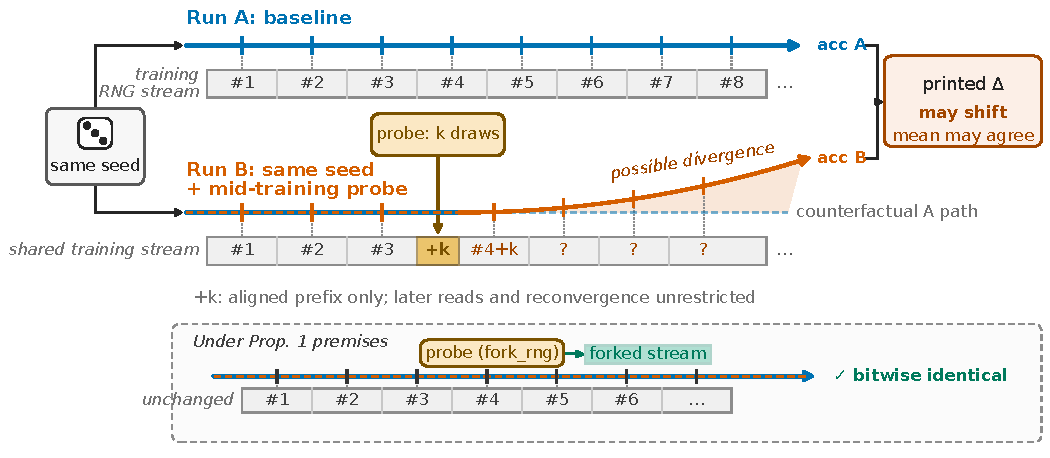
\includegraphics[width=\textwidth]{figs/fig1_mechanism.pdf}%
}{%
  \fbox{\parbox[c][2.97cm][c]{0.9\textwidth}{\centering
    Placeholder for \texttt{figs/fig1\_mechanism.pdf}.}}%
}
\caption{An extra shared-stream consumption shifts corresponding reads on the
aligned execution prefix. The first changed training-state update breaks
trajectory identity; different draws alone need not do so, and later
reconvergence is possible (Proposition~\ref{prop:pairing}). State-pure isolation
of every relevant stream restores the sufficient pairing condition.}
\label{fig:mechanism}
\end{figure}


% SOURCE: docs/PAPER_DRAFT_INTRO_DIAGNOSIS.md §3 + T4 repairs (Prop 1
% guarantee-iff, cursor streams, state purity; Prop 2 exact c_m) + T5 pins
% (+2.88 definition, probe count) + P13 verdicts + E1/E3 additions.
\section{The Pairing-Divergence Artifact}
\label{sec:f2}

\subsection{Mechanism}

The evaluation question is whether a same-seed comparison preserves the
intended control over training randomness.
Consider two runs launched from the same seed: a method arm $M$ and a
baseline arm $B$. Both draw from process-global RNG streams (PyTorch CPU,
per-device CUDA, NumPy, Python's built-in random). Suppose $M$ executes a probe
at step $t$ that consumes $k$ draws from stream $\sigma$ (a meta-validation
draw, a shuffled evaluation loader, a model re-initialization) and $B$ does
not. If training itself consumes $\sigma$
after $t$, its reads are index-shifted by $k$ on the initially aligned,
equal-consumption prefix, absent further differential consumption, restoration,
or reseeding.
Batch orders or dropout masks can change; the runs remain aligned until an
actual state update differs. Later re-coincidence is not ruled out;
the witnesses document divergence at checked checkpoints or endpoints, not every-update persistence. Single-bit differences are known to drive optimization to
materially different final models \citep{summers2021nondeterminism}; this is a
point-level effect, not a rounding curiosity. Its consequences split by estimand rather than by implementation label.
Without selection, the first failure is loss of the common-random-number
coupling (and hence of the covariance term that can reduce paired variance);
it is not, by itself, a claim of marginal mean bias. Selection on the affected
quantity is different: expected optimism relative to the selected placement's
own mean is nonnegative. The max-minus-placement-average uplift also includes
selection among unequal placement means. In our in-house predecessor a paired RTE
gain of $+2.97$ (4/5 seeds) collapsed to $+0.16$ (2/5) under isolation. That
pair predates the protocol of Section~\ref{sec:repair} and carries no verified
repeat floor (the $+2.97$ arm is by construction the unisolated one), so we
report it at a lower tier than the paper's floor-verified paired results.
Figure~\ref{fig:mechanism} sketches the mechanism.

To keep these claims separate, let $U\sim P$ denote the complete
training-visible random input for one seed and let $Y_M(U)$ and $Y_B(U)$ be
the two endpoint metrics under the intended common input. The marginal method
effect is $\tau=\mathbb E_P[Y_M(U)]-\mathbb E_P[Y_B(U)]$, whereas the paired
estimator uses $Y_M(U)-Y_B(U)$. A displaced arm observes
$\widetilde\Delta=Y_M(TU)-Y_B(U)$ for a stream-shift map $T$, and therefore
\[
\mathbb E[\widetilde\Delta]-\tau
 =\mathbb E_P[Y_M(TU)]-\mathbb E_P[Y_M(U)],\qquad
\operatorname{Var}(\widetilde\Delta)
 =\operatorname{Var}(Y_M(TU))+\operatorname{Var}(Y_B(U))
 -2\operatorname{Cov}(Y_M(TU),Y_B(U)).
\]
Thus a measure-preserving shift ($T_\#P=P$) leaves the marginal mean
unchanged but can reduce the covariance benefit; a finite data-cursor shift
need not be measure-preserving, so Proposition~\ref{prop:pairing} alone does
not assert marginal unbiasedness. For $m$ placements, the pathwise selection
uplift is $H=\max_j\Delta_j-m^{-1}\sum_j\Delta_j\ge0$; calling it a bias
requires the placement average to be the reference estimand. When selection
uses a validation quantity and reporting uses an untouched test quantity, no
one-sided conclusion follows without a transfer assumption.
\subsection{An exact condition}
\label{sec:condition}

The artifact is governed by shared stateful consumption, and the condition
is testable. We state it over \emph{streams} in a deliberately broad sense:
any shared stateful sequence with a monotone cursor, covering PRNG streams and
shared data iterators alike.

\begin{proposition}[Pairing condition]
\label{prop:pairing}
Let $X$ be the complete non-stream training state, including parameters,
buffers, optimizer and scheduler state, modes, caches, and control state;
stream values and cursors are tracked separately. Consider deterministic
executions of the same training program, initially identical in both kinds
of state, with aligned training operations $X_{n+1}=F_n(X_n,z_n)$, where
$z_n$ comprises the stream values read by operation $n$. A \emph{probe}
leaves $X$ unchanged and can affect training only through stream cursors.
Then (i) identical training reads imply bitwise-identical $X$ trajectories;
disjoint probe streams or complete fork--restore suffice. (ii) A probe
advancing one stream by $k\ge1$ shifts its subsequent training reads by $k$
only along an aligned, equal-consumption prefix with no further differential
advance, restoration, or reseeding. The first divergence is the first aligned operation
with common input state $x$ and $F_n(x,z)\ne F_n(x,z')$, not merely different
intermediate values. Later reconvergence is possible. A probe affecting only
streams never subsequently read by training is inert. (iii) Preserving reads
is sufficient, not necessary: distinct read values can induce the same state
update. No necessity or probability-one divergence claim is made.
\end{proposition}

Figure~\ref{fig:hf-boundary} is the paper's cleanest test of
Proposition~\ref{prop:pairing}, because it varies only the probe inside an
unmodified standard framework and reads the result at the bit level. The
matched five-arm audit runs inside the HuggingFace Trainer
\citep{wolf2020transformers} (RoBERTa-base, RTE, 150 steps, deterministic
kernels). Relative to the same reference, an independent repeat, Trainer
periodic evaluation (a sequential sampler and a no-grad forward), and a
CPU random-batch probe remain bitwise identical
(Figure~\ref{fig:hf-boundary}A). Only the CUDA random-batch probe diverges,
because training's dropout later consumes that same stream. A third probe
scheduled after the final update is exactly inert, realizing the boundary case
of Proposition~\ref{prop:pairing}(ii). The reason the evaluation arm survives is
\emph{stream disjointness in this configuration}, not zero consumption: the
eval loader's iterator does draw one 64-bit value from the global CPU stream
at construction (\code{torch/utils/data/dataloader.py:706--710}), the same
draw the BHN witness below turns into a divergence, but training's randomness
here lives on CUDA and on a sampler with its own generator, so no training read
is displaced. The CPU-probe arm measures that directly. A configuration whose
training path did read the global CPU stream, a stochastic collator, or another
RNG-consuming evaluation path need not be clean.

The same experiment answers how large the displacement is.
Across five seeds on each of RTE and MRPC, every CUDA-probe pair diverges and
every independent repeat remains exact (Figure~\ref{fig:hf-boundary}B). The ten
unique task--seed pairs have maximum parameter differences
$5.38$--$6.33\times10^{-4}$ (mean $5.92\times10^{-4}$). Their descriptive
$|\Delta\mathrm{acc}|$ averages $2.58$ points and reaches $5.86$, with
inconsistent sign (4 positive, 6 negative): the artifact does not merely
inflate or deflate, it scatters. At full training length the displacement
persists (Figure~\ref{fig:app-persistence}: mean $1.27$, maximum $2.73$
points), the same order as, and often
larger than, the gaps that method-comparison tables in this literature are
built on.

% Figure 3: empirical HF boundary (single column, 3.3125in).
\begin{figure}[t]
\centering
\IfFileExists{figs/fig3_hf_boundary.pdf}{%
  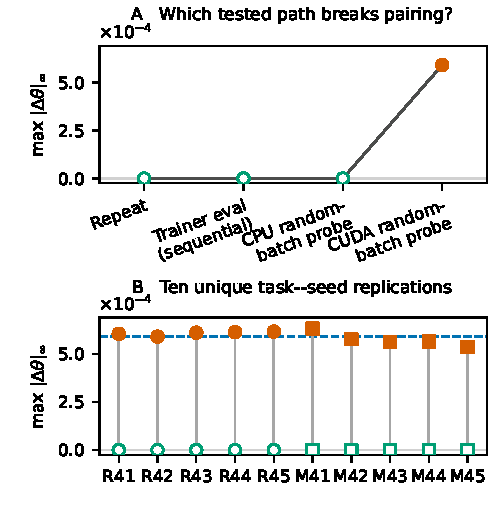
\includegraphics[width=\figwidthcol]{figs/fig3_hf_boundary.pdf}%
}{%
  \fbox{\parbox[c][2.4cm][c]{0.9\columnwidth}{\centering
    Placeholder for \texttt{figs/fig3\_hf\_boundary.pdf}.}}%
}
\caption{\textbf{Among the tested HuggingFace paths, only the probe that touches
training's CUDA random stream breaks exact pairing.} (A) In one matched
five-arm audit, repeat, sequential Trainer evaluation, and a CPU random-batch
probe are exactly zero; the CUDA random-batch probe is nonzero. (B) Across ten
unique task--seed pairs (R = RTE, M = MRPC; digits give the seed), every
repeat is exact and every CUDA probe diverges.
Each value is measured against its corresponding reference; no isolated-HF arm
is implied.}
\label{fig:hf-boundary}
\end{figure}

\subsection{Prevalence, and four byte-level witnesses}
\label{sec:prevalence}

We audited eleven published or field-standard codebases, spanning the
noisy-label and bilevel neighborhood where the diagnosis arose plus
nanoGPT as a reference pretraining loop, in two static-reading waves
(six classic repositories, four official, ${\sim}4{,}400$ stars; five
recent or large-scale). Table~\ref{tab:audit} sketches the verdicts; the
appendix gives file-line citations against pinned commits.

These eleven were \emph{chosen}, not sampled. They are the neighborhood the
diagnosis came from plus a reference pretraining loop, selected because we had
reason to suspect them. Eleven of eleven therefore measures how uniform the
idiom is inside a suspected neighborhood; it is not an estimate of any rate
across deep learning, and no count here is one. The later waves were selected the
same way, for their reach. What the audit does support is narrower: the pattern is
easy to find in code people use, no repository in the core wave isolates any
stream, and the exposure survives into work published through 2024.

The paper's evidence comes at three strengths and Table~\ref{tab:audit} sits in
the middle. \emph{Proven generally}: Proposition~\ref{prop:pairing} holds for
any run meeting its premises. \emph{Shown dynamically}: realized divergence,
confirmed by paired re-execution for four systems only; the tier column marks
which. Those four are not interchangeable either, and we rank them here rather
than let the count stand for them: Meta-Weight-Net and the new nanoGPT
campaign compare repaired arms against a \emph{probe-free} baseline; BHN and DivideMix
verify exact same-configuration floors but contrast two configurations, and
DivideMix's one line moves the mixture's initialization as well as its stream
position; the historical 200-iteration nanoGPT witness had exact floors but
no repaired arm. \emph{Static, and only that}: an EXPOSED verdict says a shared-stream
training consumer and a mid-training consumer of that stream are both present
in the source. It says nothing about whether a published number is wrong, and
nothing about any particular comparison, because desynchronizing a pair
additionally needs that consumer to fire \emph{differently} between the arms.
Where it fires identically in both, the shared stream is a path this comparison
does not walk. Arm-differential firing is what the four re-executed witnesses
show and a static reading cannot. The harvest measurements of
Section~\ref{sec:harvest} distinguish historical single-codebase calibration
from a separate nanoGPT calibration/held-out check.

\begin{table}[t]
\centering
\scriptsize
\setlength{\tabcolsep}{2.2pt}
\begin{tabular}{@{}p{0.33\columnwidth}p{0.49\columnwidth}p{0.12\columnwidth}@{}}
\toprule
Codebase & Exposure mechanism & Tier \\
\midrule
L2RW official (ICML'18) & eval consumes train iterator & static \\
L2RW PyTorch reimpl. & per-step re-init; shuffled eval & static \\
MW-Net official (NeurIPS'19) & per-step re-init + meta loader & \textbf{dyn.} \\
DivideMix official (ICLR'20) & unseeded GMM $\leftrightarrow$ mixup & \textbf{dyn.} \\
Co-teaching official (NeurIPS'18) & eval-active dropout (CUDA) & static \\
MAML reimpl. \citep{finn2017maml} & mid-epoch shuffled test loader & static \\
RENT official (ICLR'24) & on-device multinomial (CUDA) & static \\
BHN official (ICML'23) & per-epoch loader rebuild + probe & \textbf{dyn.} \\
TopoFilter official (NeurIPS'20) & per-epoch probe over shuffled loader & static \\
CRUST official (NeurIPS'20) & train-mode gradient probe & static \\
nanoGPT (60.7k$\star$) & eval shares training's randint & \textbf{dyn.} \\
\bottomrule
\end{tabular}
\caption{Eleven audited codebases, eleven exposures; none isolates any
stream (negative grep, independently re-verified); ``dyn.'' = divergence
confirmed by re-execution.}
\label{tab:audit}
\end{table}
All eleven are exposed; none
constructs a dedicated generator object to isolate any stream (verified by
negative grep), and seeding, where attempted, is a single global call
(one reimplementation never seeds torch; CRUST \citep{mirzasoleiman2020crust} defaults to none). Every
verdict was re-derived by an independent second reading against
pinned commits (SHAs in the appendix): none refuted, two strengthened, since
TopoFilter's \citep{wu2020topofilter} probe consumes a full shuffled-loader permutation per
epoch, and stock DivideMix never seeds NumPy, so exact same-seed reruns
of the released code are irreproducible past warm-up. Four of the
eleven (Meta-Weight-Net, nanoGPT \citep{karpathy2022nanogpt},
DivideMix, and BHN) are
additionally confirmed by dynamic paired re-execution (the L2RW
reimplementation was re-executed only for signal-scale measurements, not a
paired-divergence test), and in all four, paired runs diverge exactly when the
static analysis predicts. Divergence and repair are separate results, verified
on different sets, and we state the split rather than average over it.
For Meta-Weight-Net, a repaired arm run against a \emph{probe-free}
baseline was found SHA-256 identical to it (5/5 seeds). For
BHN and DivideMix we re-executed a repaired arm and verified its
same-configuration floor exactly, but the reported contrast is between two
configurations rather than against a probe-free run. The historical nanoGPT
witness had no repaired arm; the new campaign below adds that comparison.
The DivideMix witness localizes the cause to one
line: four arms of the official code (CIFAR-10, 50\% symmetric noise, 12
epochs) under one byte-identical harness that seeds NumPy and pins kernels,
neither of which the release does, differ only in whether the co-divide GMM
draws its initialization from the shared global NumPy stream or from a pinned
sklearn random state. Both repeat floors are exact; all four logs are
byte-identical through the ten warm-up epochs, where the differing line
never executes, then separate at the first co-divide epoch, ending
$0.73$ points apart on the printed final accuracy. This localizes the cause to
that line and no further: pinning the mixture's random state changes its own
initialization as well as where its draws come from, so the two arms differ
both in the split the mixture produces and in the stream position training
inherits. DivideMix is therefore a witness that the line matters, not a clean
separation of cursor displacement from re-initialization; the state-pure probes
of Proposition~\ref{prop:pairing} are the other three. The BHN witness isolates a
still smaller consumption: the single 64-bit
seed its mid-training test loader draws when its iterator is constructed
(the loader is unshuffled and eval-mode; that seed is its \emph{only}
shared-stream draw). One native generator argument to that loader removes
exactly that draw, method semantics untouched. In four arms (official
ResNet-34, CIFAR-10, 12 epochs; both repeat floors weight-exact),
per-epoch weight hashes are identical through epoch 1 and diverge exactly
at epoch 2, the first epoch whose shuffle order the probe's stream
position can reach, ending $1.93$ points apart on the printed test
accuracy: a single 64-bit draw, in official ICML-2023 code. The same
witness holds at the \emph{full shipped $200$-epoch protocol}: the
isolated pair stays bitwise-identical through all $200$ epochs, and the
configurations end at $82.68$ vs.\ $83.03$. The gap narrows to $0.35$
points but the mechanism is intact at convergence. The fourth witness
leaves supervised vision entirely: four nanoGPT arms at $200$ iterations
(\code{shakespeare\_char}, fp32) differ only in whether the loss-estimation
pass draws its batches from the same \code{randint} stream training uses,
both same-configuration repeat floors are exactly zero, and the
evaluation-versus-no-evaluation contrast reaches
$\max|\Delta W| = 3.3\times10^{-2}$ (floors in Table~\ref{tab:floors}).

Three structural observations follow. First, within this neighborhood the
pattern is structural, not incidental: the bilevel implementations draw meta-batches from a
shuffled loader on the global generator and rebuild the network
every step, so the probe fires \emph{every training step}; the artifact is a
property of the method as implemented, not of an evaluation harness. Second,
the mechanisms are diverse enough to defeat spot-checking: a data-pointer
variant needing no RNG at all (official L2RW's evaluation consumes batches from
\emph{training's own iterator}, and its pipeline re-seeds from entropy, so its
same-seed-list comparisons were never seed-controlled), an eval-active-dropout
variant (Co-teaching), and a variant whose shared draws are on the CUDA
stream (RENT). Third, the pattern
persists unchanged into ICML 2023, ICLR 2024, and the 60.7k-star reference
pretraining loop.

The reach extends past the noisy-label neighborhood, and divides along the
isolation boundary of Section~\ref{sec:repair}. A second wave reads twelve
field-standard training loops at file--line resolution
(Table~\ref{tab:fieldwide}). Ten are exposed: the reference vision recipe (timm
\citep{wightman2019timm}, whose periodic validation desynchronizes the next
epoch's shuffle, reproduced under torch~2.11), a widely copied diffusion
template \citep{lucidrains2020ddpm}, single-file RL, LLM finetuning, five
recent selection methods (Sel-CL, MLC, ProMix, UNICON, DISC), and InfoBatch:
its NumPy pruning reseed does not protect main-process torch augmentation
from the unshuffled evaluation loader's base-seed draw. Two guard the audited
RNG channel (a fixed-noise DCGAN buffer and deterministic Stable-Baselines3
evaluation with a separate, privately seeded environment); this does not
certify state purity, since DCGAN visualization updates BatchNorm buffers. A third wave
probes five flagship 2023--2026 stacks, where the boundary is a design choice
rather than an era: SDXL's in-loop logging is exposed by default; in TRL and a
diffusers script a single flag decides between exposed and guarded; OLMo-core
and MMSelfSup guard the audited RNG paths under their stated configuration conditions.
Neither wave enters the eleven-of-eleven count.

\subsection{The printed gap moves, and selection harvests it}
\label{sec:harvest}

Prevalence shows preconditions; a moved gap and a harvested one show
consequence. The
claim is tiered like the evidence: the static audit establishes the
\emph{precondition}, the byte-level witnesses the \emph{desynchronization},
the harvest the \emph{uplift in the selected reported quantity}. We claim
no audited paper's published result is wrong, only that the instrument
can be silently defeated, and that selection on the reported quantity can
produce a one-sided reported uplift. In Meta-Weight-Net's official codebase, with model,
meta-network, and RNG topology untouched and the repeat floor weight-exact
(model and meta-network SHA-identical across same-seed reruns, five seeds),
we insert one semantically inert random-permutation draw during
training and recompute the method-versus-baseline gap the paper's tables
would print. The gap moves by 1.78 points on seed 1 and 1.16 points on seed
2, in opposite directions. We make no claim about MW-Net's true ordering
against its baseline (our protocol is shortened); the claim is that in a
NeurIPS-published method's official code, a single RNG draw moves the
printed comparison by more than a point above an exact floor.

% Figure 2: harvest scatter + extreme-value growth. Rendered two-up at the
% full 6.5in measure, so it is placed at its native width and not scaled.
% Falls back to the shared column width anywhere that does not define this.
\providecommand{\figwidthharvest}{\figwidthcol}
\begin{figure}[t]
\centering
\IfFileExists{figs/fig2_harvest.pdf}{%
  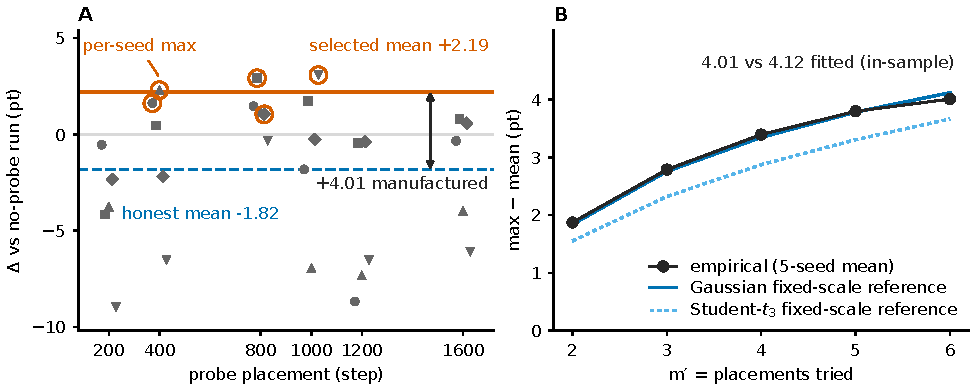
\includegraphics[width=\figwidthharvest]{figs/fig2_harvest.pdf}%
}{%
  \fbox{\parbox[c][2.97cm][c]{0.9\columnwidth}{\centering
    Placeholder for \texttt{figs/fig2\_harvest.pdf}.}}%
}
\caption{\textbf{Selection turns bidirectional divergence into a one-sided report.}
Across five seeds and six probe placements, the honest mean is $-1.82$ points,
whereas selecting each seed's best placement reports $+2.19$, manufacturing
$+4.01$. The growth over the number of tried placements tracks the finite-$m$ Gaussian benchmark in this grid rather than its asymptotic form
(Proposition~\ref{prop:harvest}). This historical grid comes from one codebase
on one dataset, with $c_m\sigma$ serving as a conditional, same-sample
benchmark whose predictive scope is assessed separately.}
\label{fig:harvest}
\end{figure}

To quantify the reporting consequence of placement selection, we use an
idealized scaling benchmark: under the iid-Gaussian null, selection over
placements has expected uplift $c_m\sigma$. Its empirical calibration is
setting-specific. The historical measurements use one codebase
(Meta-Weight-Net's official release) and dataset (CIFAR-10). The separate
nanoGPT check below estimates its own scale from calibration seeds before
held-out evaluation, assessing within-setting prediction rather than
transfer across architectures, datasets, or tasks.
Across 5 seeds $\times$ 6 placements on the same machine
(shortened protocol: Meta-Weight-Net official code on a $10{,}000$-image
CIFAR-10 subset at $40\%$ symmetric noise, $20$ epochs of $100$ steps, giving
mean within-seed sample SD $\bar\sigma = 3.25$ points, computed across
placements with denominator $m-1$ (\code{ddof=1}); Figure~\ref{fig:harvest}),
the probe \emph{hurts} on
average (honest mean $-1.82$) yet per-seed best-placement selection
reports $+2.19$, an observed $+4.01$ uplift over the placement average.
The decomposition below separates reporting optimism from systematic
placement effects; these five seeds do not identify their population shares.

\begin{proposition}[Harvest size]
\label{prop:harvest}
For integrable paired gaps $D=(D_1,\ldots,D_m)$, set $\mu_j=\mathbb E D_j$
and let $J$ be a fixed tie-broken maximizer of $D_j$. With arbitrary means
and dependence, selected-placement optimism satisfies
\[
\mathcal O:=\mathbb E[D_J-\mu_J]
\ \ge\ \max_j\mu_j-\mathbb E\mu_J\ \ge\ 0.
\]
The reported uplift $H(D)=\max_jD_j-m^{-1}\sum_jD_j$ instead obeys
$\mathbb EH(D)=\mathbb E[\mu_J-\bar\mu]+\mathcal O$; the first term need
not be positive. Common additive components cancel from $H$.
In the equal-mean Gaussian special case $D_j=a+C+\sigma Z_j$, with $\sigma\ge0$,
integrable common $C$ and i.i.d.\ standard normals $Z_j$,
$\mathbb EH=\mathcal O=c_m\sigma$, where $c_m=\mathbb E\max_j Z_j$
($c_6=1.27$). These are classical selection and order-statistic identities,
not a new universal Gaussian law.
\end{proposition}

\evidencefloats{}
The descriptive comparison is $\RevHarvest$ points of observed uplift
against $c_6\bar\sigma=\RevPrediction$, using the same placement outcomes
to estimate $\bar\sigma$, the mean within-seed sample SD. Under the
equal-mean iid-normal model, dividing each SD by its normal expectation
factor $c_4(m)$ gives $\RevCorrectedPrediction$. Exact quadrature yields
uncorrected ratios $0.9734$, $1.1463$, $1.0075$ across the shortened,
realistic-evaluation and full-best campaigns; the corrected ratios are
$0.9262$, $1.0775$, $0.9282$. Figure~\ref{fig:ratios} jointly recomputes
numerator and denominator over every ordered whole-seed bootstrap sample.
The corrected full-best interval is $[0.8665,0.9776]$: it excludes one, but
27 resamples of three seeds are a discrete sensitivity analysis, not reliable
model rejection or calibrated population coverage.

The placement effect reported at $p=0.049$ in Appendix~C relies on exchanging
fixed training positions and is conditional on that exchangeability null.
Treating observed column means as fixed offsets changed a legacy simulation
ratio from $1.00$ to $1.04$; this is a fitted-offset sensitivity, not proof
that the iid formula tolerates offsets. Appendix~C now gives a distribution-free
offset bound and a variance decomposition showing exactly how offsets and
contrast covariance enter the fitted scale.

We additionally simulate the complete fit-and-select procedure, re-estimating
all SDs in each of 100,000 Gaussian and variance-matched $t_3$ datasets.
For the $5\times6$ design, the corrected-ratio reference intervals are
$[0.8087,1.1979]$ and $[0.7251,1.3014]$, respectively. Their overlap shows
why comparing expected-maximum constants with a fixed fitted SD cannot
establish the residual distribution. The earlier growth curve is retained as
a same-grid descriptive comparison, not distributional or predictive validation.
The
harvest is consistent with an extreme-value benchmark for divergence noise,
but Proposition~\ref{prop:pairing}(ii) alone implies neither a fresh-seed law
nor Gaussian or independent placement residuals. Three limits bound how far
the agreement may be read. $c_m\sigma$
prices what a \emph{reporting practice} harvests on average over seeds rather
than what any one run will show. $\sigma$ is heteroscedastic across seeds
($1.4$--$4.6$) and does not transport between them, so a preregistered
leave-one-seed-out test misses a held-out seed's harvest by $2.17$ points on
average\evidencefigs{}. And Proposition~\ref{prop:harvest} prices selection
performed \emph{on the affected quantity}: where a validation quantity selects
and an untouched test quantity is reported, the direction and magnitude of transfer remain unestablished
by the present evidence. The preregistered bridge gives a selected
test delta of $+\RevEOneMean$. Its original preregistered seed-level $t$
interval is $[\RevEOneTLow,\RevEOneTHigh]$; the separate reviewer-requested
100,000-draw seed-cluster bootstrap gives
$[\RevEOneBLow,\RevEOneBHigh]$, also including zero. The within-seed
centered correlation is $\RevEOneR$ (Table~\ref{tab:e1}); centering removes
all seed means and does not identify the baseline's causal contribution.
We therefore
claim a guaranteed nonnegative expected optimism only for selection on the
reported quantity itself. Positive validation--test Pearson correlation
alone does not guarantee positive test-selection optimism (Appendix~C).

The mechanism also appears with an unmodified shuffled monitoring loader
(MW-Net, $45{,}000$ training images, $12$ epochs): its two seed draws
produce $+0.45$ points of max-minus-mean uplift across five seeds and five
placements. The two directly checked isolated model/meta-network pairs
match the never-probed baseline. At the full $120$-epoch protocol,
all twelve shared placement--seed pairs diverge; best-of-four uplift is
$+0.16$ points, and the three checked repaired pairs match baseline.
These are scoped endpoint comparisons, not all-placement trajectory
verification; best and final are endpoints of the same three-seed campaign.
Appendix~\ref{sec:extended-harvest} preserves the protocols, effect sizes
and verification details; Figure~\ref{fig:ledger} records the coverage.

\paragraph{Independent-setting, frozen nanoGPT prediction check.}
A separate 2,000-update campaign uses five prespecified probe placements
($200,500,900,1300,1700$), 16 calibration seeds and 16 disjoint held-out seeds.
For each seed, $D_j=L_{\rm baseline}-L_{{\rm shared},j}$ uses the same fixed
validation panel, and $H=\max_jD_j-\bar D$. Calibration alone fixes
$c_5\overline{s}/c_4(5)=0.00388406$ loss units before held-out runs;
the observed held-out mean is $0.00343060$. Independently bootstrapping
whole seed vectors in each split (20,000 draws) gives approximate 95\%
intervals $[0.00327501,0.00449714]$ for the prediction and
$[0.00279334,0.00407564]$ for the observed mean. Observed minus predicted
is $-0.00045346$ ($-11.67\%$), with interval
$[-0.00134285,0.00043370]$. Inclusion of zero establishes neither equivalence
nor the conditional Gaussian model. This is a new setting's held-out
mean-prediction check, not validation-to-test transfer or a per-run forecast.
All 160 seed--placement shared paths diverge and all 160 isolated paths
match their probe-free baseline at the checked state resolution; two
repeats per path are verification, not additional independent observations.
Appendix~\ref{sec:nanogpt-supplement} reports the prespecified uncorrected
sensitivity and exploratory selected-score, placement and influence checks.

\subsection{Kernel nondeterminism, and the repair protocol}
\label{sec:repair}

Closing every shared-stream leak is still not sufficient for pairing. With
identical training mathematics and no RNG sharing, nondeterministic GPU
kernels alone bifurcate same-seed cross-arm trajectories, a documented
layer \citep{zhuang2021randomness} for which we claim no novelty, and one
that repeat checks help distinguish from deterministic stream displacement:
a nonzero same-configuration floor detects nonrepeatability, whereas a
deterministic stream shift can leave repeats exact while moving a cross-arm
pair. A finite zero floor does not rule out all nondeterminism. The layer
is material: in an under-tuned CIFAR-100 regime
(constant lr, no augmentation, TF32), same-seed raw candidates across arms
differed by up to 11.7 points; in our NLP suite, trajectories that were
bitwise-identical for the first half epoch subsequently bifurcated by 13.7
points on CoLA. Seeds alone therefore never
establish exact pairing; repeat checks must accompany the isolation and
state-purity premises.
The repair has three requirements with different costs, and they are
checkable in the order given. Probe isolation is often a small code change;
deterministic kernels, per-path reruns, state capture, and storage can carry
substantial runtime or platform costs.

\begin{enumerate}\itemsep1pt\parskip0pt\topsep2pt
\item \emph{Isolate every probe.} Each mid-training consumer of randomness runs
inside PyTorch's fork-rng context manager \citep{pytorch_forkrng} or uses
dedicated generator objects, leaving \emph{all} training streams untouched.
All of them means all: fork-rng covers only torch's CPU/CUDA generators, so
NumPy, Python's built-in random, and library-internal draws need dedicated or
pinned states (DivideMix's repair pins sklearn's); a shared \emph{data cursor}
needs its own iterator (official L2RW consumes no RNG at all); and the probe
must write no training-visible state, state purity in the sense of
Proposition~\ref{prop:pairing}. Figures~\ref{fig:hf-boundary}
and~\ref{fig:app-realeval} show the boundary this draws.
\item \emph{Pin kernels.} Deterministic kernels for any run used in a paired
claim; nondeterministic ones break pairing with no RNG sharing at all.
\item \emph{Verify a zero repeat floor on every materially distinct path.}
Rerun each arm and configuration whose kernel, control flow, precision,
stochastic consumer, or probe differs, under the identical seed and
configuration. Require the difference to be exactly zero at the resolution of
the intended claim before interpreting a cross-arm delta (per-campaign floors:
Table~\ref{tab:floors}). A metric floor supports only a metric claim; weight
or full-state claims require the corresponding hashes. The floor turns ``we
set seeds'' into a measurement on the tested path, not a universal proof of
determinism.
\end{enumerate}

\noindent In released code the first requirement is often a small wrapper, and the
three systems where we re-executed a repaired arm show the shape of it.
Meta-Weight-Net's per-step probe needs the probe body wrapped in
\code{with torch.random.fork\_rng(devices=[device]):} (\code{devices=[]} on
CPU), after which the isolated arm
is SHA-256 identical to the never-probed baseline on 5/5 seeds. BHN's
mid-training test loader draws one 64-bit seed at iterator construction, removed
by passing \code{generator=torch.Generator().manual\_seed(0)} to that
\code{DataLoader}, method semantics untouched. DivideMix's co-divide GMM draws
from global NumPy, pinned by \code{GaussianMixture(..., random\_state=0)}. Each
exposure in the field-wide wave maps to one of those three shapes, a
\code{fork\_rng} wrapper for an in-loop evaluation or sampling call, a
dedicated \code{generator=} for a probe's loader, or a pinned state for a
library that reads a global stream. Apart from the new nanoGPT campaign
above, we have not re-executed repaired arms in that wave; for those
remaining entries the mapping is a prescription, not a result.

\noindent Table~\ref{tab:floors} records the actual repeat evidence and its
resolution, including absent floors. Historical NLP zero cells and the
pre-protocol in-house comparison are excluded from certificate counts.
A floor from one tested path is not silently transferred to a distinct arm.
The isolation clause is verified on the witness codebase itself:
fork-rng isolation returns model and meta-network to SHA-256 identity with
the never-probed baseline, on five seeds at the shortened protocol and three
at the full (probes verified to fire).

\subsection{The repair's certificate: a certified no-op}
\label{sec:receipt}

The repair gives a conditional no-op result, illustrated by a guarded
weight-averaging endpoint that may serve its raw candidate. Candidate
maintenance and evaluation must satisfy Proposition~\ref{prop:pairing};
repeat floors test the implementation but do not replace its premises.

\begin{corollary}[Certified no-op]
\label{cor:noop}
Under the deterministic pairing protocol, state-pure and stream-isolated
candidate maintenance gives champion $=$ raw $\Rightarrow$ served parameters
and buffers are bitwise identical to the paired baseline endpoint, so every
deterministic reported metric delta is exactly zero. The reverse implication
requires the additional checked premise that every non-raw candidate differs
from raw in at least one parameter bit; EMA or frozen candidates may collide
exactly and this premise is not inferred merely from training having moved.
\end{corollary}

The certificate requires the full conjunction of premises, not merely a
logged raw champion and a zero metric. Historical tuned-regime observations
are retained in Table~\ref{tab:certreg} as descriptive results, with missing
floors excluded from certificate counts. Direct weight comparisons, metric
equality and full-state verification remain distinct evidence categories
(Figure~\ref{fig:ledger}). Detailed averaging, monitor and meta-signal analyses
are in the appendix; the main contribution is the pairing diagnosis and
the operational checks that make its repair testable.


% Diagnosis II used to be a body section here. It is now appendix-only (see the
% \diagtwoscope / \contribdiagtwo macros above): a correct result on a thinner
% evidence base than the audit, which reviewers read as a second, loosely
% attached paper when it sat in the body. sections_tmlr/f1.tex is retired; the
% appendix is the single source.

\begin{figure}[t]
\centering
\IfFileExists{figs/fig_r3_evidence_ledger.pdf}{%
  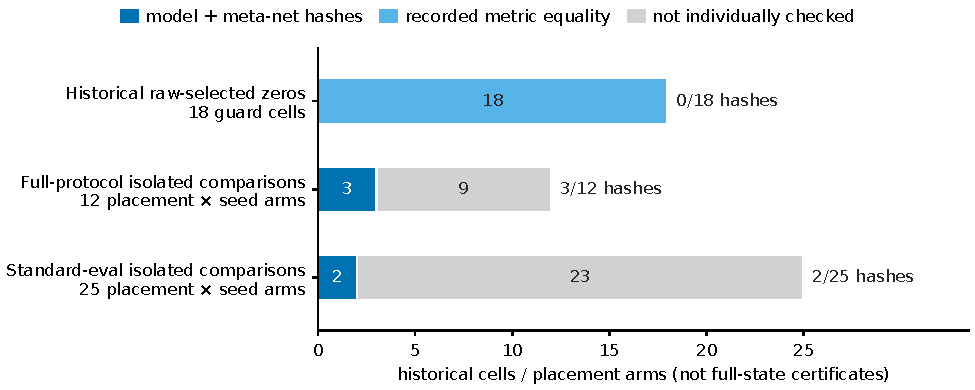
\includegraphics[width=\textwidth]{figs/fig_r3_evidence_ledger.pdf}%
}{}
\caption{Verification resolution, separated from certificate eligibility.
The full-protocol and realistic-evaluation cure counts are reproduced from
archived model and meta-network hash pairs (3/12 and 2/25). Historical guard
metrics and text-reported checks do not establish a full-state certificate;
cells without independent floors are excluded from certificate counts.
Unmeasured repaired arms remain unverified, not inferred successes.}
\label{fig:ledger}
\end{figure}

\section{Related Work}

Common-random-number alignment is established in stochastic simulation
\citep{glasserman1992crn,stout2008keeping,pearce2022bayesian}.
Recent work quantifies variance reductions from alignment
\citep{klein2024noisefree} and repairs intervention-induced stream shifts
with counter-based RNG \citep{buffalo2026realizing}. Isolation tools already
exist in JAX and PyTorch \citep{jax2018prng,pytorch_forkrng}.
We do not claim a new general principle of randomness or model selection:
the contribution is a deep-learning evaluation diagnosis, released-code
causal witnesses, and a connection to selection on the displaced quantity.

Deep-learning studies document sensitivity to perturbations and the need
to account for variability across seeds
\citep{summers2021nondeterminism,dodge2020finetuning,bouthillier2021accounting}.
Our question complements single-run reproducibility: can an arm-specific
operation invalidate the intended same-seed comparison?
Deterministic-execution tools
\citep{chen2022reproducible,heumos2023mlfcore,shkolnikov2026bitidentical}
help check the repair, but determinism alone does not establish cross-arm
pairing. Desynchronization need not alter the marginal mean effect; selecting
favorable outcomes on the reported quantity invokes classical selection
optimism \citep{cawley2010overfitting}.

Appendix~\ref{sec:extended-context} develops these connections, including
the reweighting methods motivating the audit and the weight-averaging
literature relevant to our conditional no-op application.

\section{Discussion}
\label{sec:discussion}

\paragraph{Evaluation practice.}
Same-seed comparisons should check the three practices in
Section~\ref{sec:repair}: isolate probes, pin kernels, and verify each
materially distinct execution path at the resolution claimed.
Stream sharing alone does not imply divergence: the tested Trainer
evaluation is configuration-specifically stream-disjoint from training
(Table~\ref{tab:hf}). Existing isolation primitives help, but their use must
be checked. Deterministic execution and repeat/state audits incur runtime
and storage costs; some platforms lack deterministic implementations.

\paragraph{Interpretation and scope.}
Desynchronization, variance changes, and selection optimism are distinct.
Observed max-minus-mean uplift can contain both systematic placement
effects and optimism; the Gaussian formula applies only under its stated
model. Omitting selection removes this source of directional optimism,
not trajectory displacement. The no-op corollary is an application of the
pairing condition, not an accuracy claim about selection or averaging.

Our evidence is single-process and academic-scale, not distributed training,
ImageNet, or production-LLM validation. The nanoGPT experiment checks a
frozen mean prediction on held-out seeds in one setting, not universal
Gaussian scaling, per-run prediction, or untouched-test transfer.
Static exposure remains distinct from dynamic evidence, and historical
score-level equality does not establish state-level identity.
Appendix~\ref{sec:extended-context} records the detailed scope and practical
limitations.

\section{Conclusion}

Matching initial seeds does not ensure aligned training randomness.
Arm-specific probes can displace later training draws; our pairing
condition guarantees preservation and localizes divergence onset on the
aligned prefix without ruling out later re-coincidence.
Released-code witnesses make this evaluation failure concrete.
Desynchronization alone need not bias the expected effect: selection on
the affected reported quantity creates a separate optimism mechanism,
while positive untouched-test transfer remains unestablished.
The general selection decomposition accommodates placement effects;
Gaussian scaling is a conditional benchmark, with a separate held-out
mean check in nanoGPT. The repair is checkable through probe isolation,
deterministic execution, and per-path repeat checks at the claimed
resolution.

% Broader Impact stays in the paper proper: TMLR expects it here, after the
% conclusion and before the references. The reproducibility statement it used
% to sit beside is not a TMLR requirement (the venue asks for reproducibility
% *material* as supplementary files), so it moved to Appendix G, with one
% pointer from the conclusion.
% SOURCE: written for the TMLR submission. Kept short and specific: the two
% concerns that are actually particular to THIS paper are naming real
% repositories and describing an exploitable procedure, so those are what the
% statement addresses rather than generic ML-risk boilerplate.
\section*{Broader Impact Statement}

This paper studies how experiments are measured rather than proposing a model,
a dataset, or a deployed system, so its effect is on research practice. Two
consequences deserve naming. First, the audit names repositories and commits:
we report structural preconditions and, where we re-executed, realized
divergence, but claim no published result is wrong. These are careful
implementations, written when nothing in the tooling or the review process
asked for probe-RNG isolation, and the same reading returned the same verdict
on our own predecessor first. Second, a procedure that inflates a reported
gap is a recipe as well as a diagnosis. Disclosure is safer: the mechanism is
already live in widely used released code, so it operates whether or not
practitioners intend it. Isolation is often a small code change, but the full
repair also requires deterministic execution and per-path repeat checks,
with runtime, storage and platform costs.


\bibliography{refs}
\bibliographystyle{tmlr}

\appendix
% The supplement is set at the document's own 10pt. It was briefly set \small
% to buy pages. Preserve the standard body font and meet the regular-submission
% limit by relocating auxiliary detail instead. Table bodies stay \footnotesize, which is
% ordinary practice and not a prose-size reduction.
% GENERATED by scripts/revision_generate_appendix.py; edit paper/appendix.tex.
\noindent The appendix is organized as follows. Appendix~A is the static-audit
register: per-repository mechanisms cited by file and line against pinned
commits, verdicts, and the corrections an independent second reading produced.
Appendix~B verifies at source level the main text's two framework claims,
the tested HuggingFace Trainer stream disjointness and Proposition~1's PyTorch stream
premises. Appendix~C proves the three propositions, the certified-no-op corollary and
the margin-calibration lemma, and states the paper's second, appendix-scoped
diagnosis in Appendix~\ref{sec:deadmeta-taxonomy}. Appendix~D gives the pairing
protocol, the per-campaign repeat-floor registry, the traced MW-Net divergence
witness, and the preregistered validation-to-test bridge; Appendices~E and~F
are the environment manifest and a note on the monitor figures. Every SHA,
citation, and quotation was read against the pinned version stated, and
main-text statements are restated before their proofs.

\section{Static Audit: Pinned Commits, Mechanisms, and the Double-Read
Register}
\label{sec:audit}

\paragraph{Tone, stated once and applying to every named repository.}
These verdicts convict a practice, not people. The audited releases are careful
implementations of influential methods, and we know of no venue checklist or
framework default from their era that asked for probe-RNG isolation. The same
reading applied to our own predecessor system returned the same verdict first.

\paragraph{Method.}
Two static-reading waves over shallow clones pinned by commit SHA: six classic
method repositories (four official releases; ${\sim}4{,}400$ stars combined;
Table~\ref{tab:classic}) and five recent or large-scale targets
(Table~\ref{tab:recent}). A third wave (Table~\ref{tab:modern}) reads five
flagship 2023--2026 stacks as a \emph{boundary probe} rather than a prevalence
claim: three-way verdicts (exposed / guarded / ambiguous with the deciding flag
stated), a single reading whose load-bearing citations were independently
re-verified against the pinned clones, entering neither the eleven-repository
count nor the corrections register. Static reading establishes only that the
consumption pattern exists, a claim about code rather than about any published
number; realized divergence comes from the re-execution witnesses, whose floors
are registered in Appendix~D, and the remaining six verdicts are labeled static
in the main text. An independent second reading against the same pinned commits
refuted 0/11, strengthened two (TopoFilter, DivideMix), and produced seven
secondary corrections, an eighth surfacing during witness construction
(register below).

\paragraph{The shared negative result.}
None of the eleven codebases constructs a dedicated \code{torch.Generator}
for any \code{DataLoader}, wraps any probe in \code{fork\_rng}, or
save-restores RNG state around any mid-training consumer; each relies on a
single global seed call (or none). For the recent five this was re-verified
in the second reading with a widened negative grep over all \code{.py}
files; the pattern
\begin{center}
\code{torch.Generator|generator=|fork\_rng|get\_rng\_state|set\_rng\_state}
\end{center}
returns zero hits, and all 14 seeding sites in those five repositories
are global \code{manual\_seed}-family calls.

\begin{table}[tbp]
\centering
\footnotesize
\setlength{\tabcolsep}{4pt}
\begin{tabular}{@{}L{2.0cm}L{1.1cm}L{5.7cm}L{1.6cm}L{3.3cm}@{}}
\toprule
Codebase (venue) & Commit & Exposure mechanism (file:line) & Verdict &
Double-read note \\
\midrule
L2RW official, TF1 (ICML 2018) & \code{0b616c9} &
Periodic eval pulls 50 batches from \emph{training's own iterator}
(\code{mnist\_train.py:396--397} $\to$ \code{:270--272}), advancing the
shared epoch cursor; \code{DataSet} construction re-seeds global NumPy
(\code{mnist/mnist.py:151--153}), whose shuffles the loaders share
(\code{:214--216}, \code{:230--232}); per-step meta-validation draw
(\code{mnist\_train.py:372--373}) &
EXPOSED (data cursor $+$ NumPy global) &
Corrected (register~1); verdict unchanged, and the
paired-in-intent reading strengthened \\
\addlinespace
L2RW PyTorch reimpl. & \code{182aad0} &
Per-step meta-network re-instantiation (notebook cell~17) draws dozens of
initialization samples from the global CPU stream; test loader shuffled by
an unconditional override (\code{data\_loader.py:105--111}); fresh
\code{iter()}, one \code{randperm}, every training step &
EXPOSED (CPU stream) &
Corrected (register~2); verdict unchanged \\
\addlinespace
Meta-Weight-Net official (NeurIPS 2019) & \code{3f1800f} &
Meta-loader iterator created before the train iterator and re-created
mid-epoch (\code{MW-Net.py:196--197}, \code{:214--218}); full model
re-instantiation every step (\code{:200--201}); meta-batch fetches advance
the shared Python-\code{random} augmentation stream &
EXPOSED (CPU stream, per step) &
Corrected (register~3); step-0 desynchronization conclusion stands \\
\addlinespace
DivideMix official (ICLR 2020) & \code{d9d3058} &
\code{GaussianMixture} fitted with no \code{random\_state}
(\code{Train\_cifar.py:186--187}) draws its initialization from global
NumPy, interleaved with training's \code{np.random.beta} mixup draws
(\code{:87}); NumPy never seeded; per-epoch loader rebuilds with
GMM-dependent split sizes (\code{:264--272}) &
EXPOSED (NumPy $+$ structural) &
Confirmed; zero-hit repo-wide grep for \code{np.random.seed}; same-seed
reruns of the stock code are irreproducible past warm-up. Subsequently
confirmed dynamically (four-arm witness, Appendix~D): pinning the GMM's
\code{random\_state} (one line) moves the final weights, with both
repeat floors exact and warm-up logs byte-identical \\
\addlinespace
Co-teaching official (NeurIPS 2018) & \code{7c7fbe2} &
Functional dropout without a \code{training} argument (\code{model.py:45},
\code{:54}) stays active under \code{model.eval()} (the API default is
\code{training=True}); the per-epoch test evaluation (\code{main.py:295})
therefore consumes the CUDA stream shared with training-time dropout &
EXPOSED (CUDA stream) &
Corrected (register~4); verdict unchanged \\
\addlinespace
MAML-PyTorch reimpl. & \code{98a00d4} &
A shuffled test \code{DataLoader} is constructed mid-training every 500
steps (\code{miniimagenet\_train.py:78--86}), drawing \code{randperm} from
the global CPU generator shared with the training loader (\code{:67}) &
EXPOSED (CPU stream) &
Confirmed; Python-\code{random} unseeded repo-wide (episode composition
itself irreproducible) \\
\bottomrule
\end{tabular}
\caption{Classic wave: six method codebases, six exposures (four official
releases; ${\sim}4{,}400$ stars combined). Static reading of pinned
commits; every verdict re-derived by an independent second reading, with
corrections listed in the register.}
\label{tab:classic}
\end{table}

\begin{table}[tbp]
\centering
\footnotesize
\setlength{\tabcolsep}{4pt}
\begin{tabular}{@{}L{2.0cm}L{1.1cm}L{5.7cm}L{1.6cm}L{3.3cm}@{}}
\toprule
Codebase (venue) & Commit & Exposure mechanism (file:line) & Verdict &
Double-read note \\
\midrule
nanoGPT (60.7k stars) & \code{3adf61e} &
The single data path \code{get\_batch} draws \code{torch.randint} with no
\code{generator=} (\code{train.py:123}); \code{estimate\_loss} reuses it
for exactly 400 draws per evaluation (2 splits $\times$ 200
\code{eval\_iters}; 4{,}800 sampled positions at batch 12); all three call
sites (\code{:222}, \code{:250}, \code{:303}) share the stream; evaluation
fires at iteration 0 as well &
EXPOSED (CPU; canonical) &
Confirmed; call-site enumeration verified exhaustive; one line range
corrected (see register) \\
\addlinespace
RENT official (ICLR 2024) & \code{d40f3c4} &
On-device \code{torch.multinomial} every training batch
(\code{method\_utils.py:122--123}) advances the global CUDA stream by a
data-dependent amount; train loader \code{shuffle=True} with no generator &
EXPOSED (CUDA escalation) &
Corrected (register~5); consumption chain additionally verified by
execution \\
\addlinespace
BHN official (ICML 2023) & \code{2b09d3a} &
The default CIFAR-10 path's train loader is built once
(\code{BHN.py:756}) and re-iterated every epoch (\code{:781}), drawing
per-sample augmentation and the loader's own shuffle seed from the global
CPU generator; every epoch ends with a mid-training test
(\code{:810}), whose \code{test\_loader} construction (\code{:209--210})
draws one further global-stream value at iterator creation with no
\code{generator=} &
EXPOSED (CPU stream) &
Corrected (register~8): the lines first cited
(\code{:407--408}, \code{:430}) belong to
\code{PvalueTrainer}\allowbreak\code{Clothing1M}, the Clothing1M path, not to the audited
default CIFAR-10 path \code{PvalueTrainer}. Verdict unchanged, and
confirmed dynamically (Appendix~D) \\
\addlinespace
TopoFilter official (NeurIPS 2020) & \code{9835d8c} &
Per-epoch feature/connected-component probe interleaved with training
(\code{train.py:227--263}); training loaders \code{shuffle=True} with no
generator (\code{:103}, \code{:350}) &
EXPOSED (CPU stream) &
Confirmed and strengthened (register~6): the probe itself iterates a
shuffled trainloader each epoch (\code{:269}) \\
\addlinespace
CRUST official (NeurIPS 2020) & \code{a430069} &
Per-epoch train-mode gradient-estimation pass and coreset re-selection
mutate the dataset the shuffled loader sees
(\code{robust\_cifar\_train.py:201--237}; loader \code{:176}); per-epoch
\code{validate()} &
EXPOSED (CPU $+$ structural) &
Corrected (register~7); default \code{--seed} is \code{None}, so default
runs are entirely unseeded \\
\bottomrule
\end{tabular}
\caption{Recent wave: five recent or large-scale codebases, five
exposures. The pattern persists unchanged into ICML 2023, ICLR 2024, and
the reference LLM pretraining loop; the same negative grep applies
(zero isolation hits across all five).}
\label{tab:recent}
\end{table}

\begin{table}[tbp]
\centering
\footnotesize
\setlength{\tabcolsep}{4pt}
\begin{tabular}{@{}L{2.0cm}L{1.1cm}L{5.9cm}L{1.6cm}L{3.3cm}@{}}
\toprule
Stack (paradigm) & Commit & Mechanism / isolation (file:line) & Verdict &
Boundary note \\
\midrule
HF TRL (RLHF post-training) & \code{b6ff4a7} &
Generation-based evaluation routes through the same
\code{generate(do\_sample=True)} as training rollouts, on the global
torch stream (\code{grpo\_trainer.py:1614}; config built \code{:959--972}
with no generator); post-generation \code{torch.randperm} unisolated
(\code{trainer/utils.py:831}). The dataloader \emph{is} isolated: a
dedicated \code{Generator} in \code{RepeatSampler}
(\code{utils.py:712--719}) &
ambiguous &
exposed on the default backend; \code{use\_vllm=True}
(default \code{False}, \code{grpo\_config.py:574}) moves generation to
an isolated engine \\
\addlinespace
AI2 OLMo-core (LLM pretraining) & \code{fa6c501} &
The in-loop evaluator forces \code{model.eval()} before every eval
forward (\code{train\_module.py:497}, \code{:649--654}), gating off the
only training-mode global draws (MoE jitter \code{router.py:331},
\code{:336}; dropout defaults off); batch order is counter-keyed from a
dedicated PCG64 generator (\code{data\_loader.py:667--688}) &
guarded &
no audited configuration flips it. The $k = 0$ counts the training-mode
global draws the evaluator gates off, not every value an evaluation path
could take; what carries the verdict is the dedicated generator, which
leaves training's batch order disjoint from the global stream whatever an
eval loader draws from it \\
\addlinespace
Stability generative-models / SDXL (diffusion) & \code{e8cd657} &
\code{ImageLogger.on\_train\_batch\_end} (\code{main.py:457--459})
samples images via \code{torch.randn} (\code{diffusion.py:246}) plus
per-step \code{randn\_like} on the global stream that training's noise
and timesteps consume (\code{loss.py:72};
\code{sigma\_sampling.py:12}, \code{:29}); negative greps:
\code{fork\_rng}, \code{isolate\_rng}, \code{torch.Generator},
\code{generator=}, RNG state save/restore all zero hits &
exposed &
on by default (\code{batch\_frequency} 1000, installed as a default
callback) \\
\addlinespace
OpenMMLab MMSelfSup (vision SSL) & \code{db861f3} &
The DeepCluster extract loader is \code{shuffle=False}
(config \code{:55}), so its \emph{sampler} draws nothing (\code{torch.arange},
mmengine \code{sampler.py:75--76}); its iterator still takes the one
\code{\_base\_seed} value on fresh iterator construction
(\code{dataloader.py:706--710}), which is harmless here only because
training shuffle uses a private
\code{Generator} (\code{deepcluster\_sampler.py:47--48}; mmengine
\code{sampler.py:72--74}); augmentation randomness is confined to
per-worker-seeded subprocesses (mmengine \code{dataset/utils.py:36--39});
persistent workers reuse existing iterators &
guarded &
the one config-gated global-NumPy draw
(\code{set\_uniform\_indices}, \code{:88}) self-reseeds per epoch and
lives in main-process NumPy, which training augmentation never reads.
The hook also updates labels and initializes its classifier; this RNG
verdict does not assert state purity \\
\addlinespace
HF diffusers (training examples, diffusion) & \code{d1b988b} &
\code{log\_validation}'s pipeline receives
\code{generator = None if args.seed is None else torch.Generator(...)}
(\code{train\_text\_to\_image.py:161--164}, consumed \code{:174});
\code{randn\_tensor} draws the global stream iff the generator is
\code{None} (\code{torch\_utils.py:232}), the stream training
consumes (\code{:972}, \code{:982}) &
ambiguous &
the boundary is exactly \code{--seed}: passed $\to$ guarded; omitted
$\to$ every validation image shifts subsequent noise and timesteps \\
\bottomrule
\end{tabular}
\caption{Third wave (boundary probe): five flagship 2023--2026 stacks
across RLHF post-training, LLM pretraining, diffusion, and
self-supervised vision. Unlike the two prevalence waves this wave makes
no all-exposed claim and its verdicts are three-way; it was a single
reading whose every load-bearing citation was independently re-verified
against the pinned clones. The split lands on the isolation primitives
of the repair protocol, and these five do not enter the
eleven-repository count.}
\label{tab:modern}
\end{table}

\paragraph{Corrections register (seven corrections from the double-read,
an eighth from witness construction; zero verdicts refuted).}
\begin{enumerate}\itemsep2pt
\item \emph{L2RW official}: provenance inversion, the executed \code{DataSet}
coming from TensorFlow r1.10 with the vendored copy dead code (mechanism
byte-identical); an \code{nval} confusion clarified. Lacking a graph-level seed
it re-seeds from entropy, so the repository's same-seed-list comparisons
(\code{mnist\_train.py:417--422}) were never seed-controlled, strengthening
the ``paired in intent, desynchronized in fact'' reading.
\item \emph{L2RW PyTorch}: periodic evaluation is cadence-symmetric across
arms; the arm-differential consumer is the per-step re-instantiation, as first
stated.
\item \emph{Meta-Weight-Net}: on \code{torch} 0.4.0 the loader-creation
\code{randperm} shift does not hold (lazy \code{BatchSampler}); the first
differential consumers are the per-step rebuild (\code{:200}) and meta-batch
augmentation (\code{:215}). The flip-noise path also ignores \code{--seed};
step-0 conclusion and verdict stand.
\item \emph{Co-teaching}: selection uses \code{np.argsort}, not
\code{torch.sort}; both RNG-free, so nothing changes. CPU-stream
non-contamination re-verified under \code{torch} 0.3.0.
\item \emph{RENT}: \code{TV.py:41}'s \code{randint} draws CPU-side then moves
to device; the CUDA draws are \code{PDN.py:191} and \code{BLTM.py:96}.
Table~\ref{tab:recent}'s headline mechanism is unaffected.
\item \emph{TopoFilter}: exposure understated, the probe itself iterating a
shuffled trainloader every epoch (\code{:269}) for a full permutation plus
augmentation draws.
\item \emph{CRUST}: facility-location weights are unnormalized counts
(\code{:215}) and \code{--seed} defaults to \code{None}, so default runs are
entirely unseeded.
\item \emph{BHN}: the lines first cited (\code{:407--408}, \code{:430}) are
the Clothing1M path; the default CIFAR-10 path exposes the same mechanism at
\code{:756}, \code{:781}, \code{:810}, later confirmed dynamically
(Appendix~D).
\end{enumerate}
One further correction is typographical and uncounted: nanoGPT's
\code{estimate\_loss} spans \code{train.py:215--228}, a one-line offset. Net:
0/11 verdicts refuted, 2 exposures strengthened, 8 mechanism-level corrections
(7 double-read, 1 from witness construction), none touching a verdict.

\paragraph{Scope of the verdicts.}
EXPOSED is a claim that the preconditions of Proposition~1(ii) are present
in the code: a global-stream (or shared-cursor) training consumer plus a
mid-training consumer of the same stream. For Table~\ref{tab:modern},
GUARDED means the probe exists but is isolated by design, and AMBIGUOUS
means exposure is decided by a stated flag or argument. None of these is,
by itself, a claim
that any specific published number is wrong, and we make no such claim for
any audited repository. Nor is any of it a rate. Every repository here was
picked deliberately, the first wave because it is the neighborhood the
diagnosis came from and the later waves for reach across eras and task
families, so the counts describe what we looked at and support no inference
to a population of repositories we did not. The realized-divergence and harvest claims of the
main text rest on the re-execution witnesses and our own campaigns;
Appendix~D records which paths have repeat floors and at what resolution.

\subsection{Second wave: field-standard training loops}
\label{sec:audit-fieldwide}

The main text's claim that the exposure reaches past the noisy-label
neighborhood rests on a second audit of twelve field-standard codebases spanning
diffusion, vision recipes, reinforcement learning, LLM finetuning, and recent
sample-selection methods. We separate it from the double-read core by
verification tier: this wave is a single structured reading at pinned commits,
of which the four headline verdicts (\code{timm}, \code{lucidrains/ddpm},
Sel-CL, MLC) were independently re-verified at file--line by the authors, and
\code{timm}'s data-order channel was reproduced empirically under \code{torch}
2.11 (inserting an eval-loader iteration between epochs shifts the next epoch's
train shuffle). Confidence is stated per row; these repositories do not enter
the eleven-of-eleven count.

\begin{table}[tbp]
\centering
\footnotesize
\setlength{\tabcolsep}{4pt}
\begin{tabular}{@{}L{2.15cm}L{1.2cm}L{8.3cm}L{1.7cm}L{1.0cm}@{}}
\toprule
Codebase (kind) & Commit & Shared-stream mechanism: training consumer $\to$
mid-training consumer (file:line) & Verdict & Conf. \\
\midrule
Sel-CL (CVPR'22) & \code{98cc41e} &
\code{WeightedRandomSampler} on global torch, no generator
(\code{train\_Sel-CL.py:193}) $\to$ per-epoch \code{pair\_selection} draws
\code{torch.rand(len(trainloader.dataset), args.low\_dim)}, $50{,}000\times128$
on CIFAR (\code{utils/utils\_noise.py:359}) &
EXPOSED & high \\
\addlinespace
MLC (AAAI'21) & \code{5747d0b} &
silver (train) loader \code{shuffle=True}, no generator
(\code{CIFAR/data\_helper\_cifar.py:76}) $\to$ per-epoch validation loader
\code{shuffle=True} (\code{:78}) draws a full global permutation &
EXPOSED & high \\
\addlinespace
ProMix (IJCAI'23) & \code{40d8378} &
mixup \code{torch.randperm} + train \code{shuffle=True}
(\code{Train\_promix.py:208}; \code{dataloader\_cifarn.py:276}) $\to$
selection \code{eval\_train} iterates a multi-worker loader
(\code{Train\_promix.py:427}), one worker base-seed draw/epoch & EXPOSED & med \\
\addlinespace
UNICON (CVPR'22) & \code{1b5a03f} &
mixup \code{randperm} + train \code{shuffle=True}
(\code{Train\_cifar.py:148}) $\to$ \code{Calculate\_JSD} eval loader
worker base-seed (\code{dataloader\_cifar.py:340}) & EXPOSED & med \\
\addlinespace
DISC (CVPR'23) & \code{a21e910} &
mixup \code{randperm} + train \code{shuffle=True}
(\code{losses/loss\_mixup.py:27}, called from \code{DISC.py:308}) $\to$
per-epoch \code{model.evaluate} loader worker base-seed (\code{main.py:204}) & EXPOSED & med \\
\addlinespace
lucidrains DDPM (diffusion, ${\sim}9$k$\star$) & \code{d93647a} &
forward-diffusion \code{torch.randint}/\code{randn\_like}
(\code{denoising\_diffusion\_pytorch.py:838}) $\to$ mid-training
\code{ema.sample()} draws \code{torch.randn} (\code{:686}, \code{:709}) on the
same global stream, default \code{every 1000} & EXPOSED & high \\
\addlinespace
timm (vision recipe, ${\sim}33$k$\star$) & \code{ce7c976} &
train loader \code{shuffle}, no generator (\code{data/loader.py:348}) $\to$
\code{validate()} (\code{train.py:1392}) advances the base seed on first
iterator construction; persistent reuse is not a fresh draw every epoch.
Nondistributed shuffle path; \emph{empirically reproduced} & EXPOSED & high \\
\addlinespace
CleanRL (RL, ${\sim}6$k$\star$) & \code{fe8d8a0} &
online $\epsilon$-greedy \code{random.random()} (\code{qdagger\_dqn\_}\allowbreak\code{atari\_impalacnn.py:362})
$\to$ periodic offline \code{evaluate} reuses global \code{random}
(\code{dqn\_eval.py:28}) & EXPOSED & high \\
\addlinespace
litgpt (LLM finetune, ${\sim}12$k$\star$) & \code{2685705} &
LoRA \code{Dropout} on global torch (\code{lora.py:82}; default
\code{lora\_dropout=0.05}, \code{finetune/lora.py:58}) $\to$
periodic \code{generate\_example} temperature sampling
\code{torch.multinomial} (\code{generate/base.py:36}); dataloader \emph{is}
guarded, generation is not & EXPOSED & high \\
\addlinespace
InfoBatch (ICLR'24, ${\sim}346$$\star$) & \code{8bbb012} &
unshuffled test loader, no generator
(\code{research/cifar\_example.py:76--77}), consumes a CPU base seed;
next-epoch random flip/crop (\code{:51--54}) runs with zero workers
(\code{:70--71}). NumPy pruning reseed does not isolate torch augmentation
& EXPOSED & high \\
\addlinespace
PyTorch DCGAN example (${\sim}23$k$\star$) & \code{acc295d} &
training \code{torch.randn} (\code{dcgan/main.py:240}) $\to$ periodic
visualization reuses a precomputed \code{fixed\_noise} buffer
(\code{:211}), drawing zero new noise. RNG-only guard: train-mode
\code{netG(fixed\_noise)} (\code{:268}) updates BatchNorm buffers & GUARDED & high \\
\addlinespace
Stable-Baselines3 (${\sim}10$k$\star$) & \code{8908708} &
rollout action sampling on global torch $\to$ \code{EvalCallback}
uses a separate \code{eval\_env} + \code{deterministic=True} default
(\code{callbacks.py:379}); assumes private environment randomness and
deterministic policy internals. Stochastic actions or custom global-RNG
components are outside this guard &
GUARDED & med \\
\bottomrule
\end{tabular}
\caption{Second-wave audit of twelve selected training loops: ten EXPOSED,
two guarded on the stated RNG channel. Re-reading the pinned InfoBatch
CIFAR path changes its earlier guarded verdict to exposed: counter-reseeding
NumPy does not isolate torch CPU augmentation from a loader base seed.
Across all 28 paths the revised counts are 22 exposed, four guarded and
two configuration-dependent. Guarded does not imply state purity or
universal framework immunity. Exact source-chain conditions and before/after
verdicts are recorded in the revision audit ledger.}
\label{tab:fieldwide}
\end{table}

\section{Framework Source-Level Verification}
\label{sec:framework}

\subsection{HuggingFace Trainer: tested stream disjointness
(\code{transformers} 5.12.1)}

The main text reports that the Trainer's built-in periodic evaluation is
bitwise clean in the five-arm experiment. That measurement has a
source-level explanation, verified against the installed
\code{transformers} 5.12.1 (quotes condensed to the load-bearing
expression).

\begin{table}[tbp]
\centering
\footnotesize
\setlength{\tabcolsep}{5pt}
\begin{tabular}{@{}L{4.6cm}L{4.4cm}L{6.3cm}@{}}
\toprule
Claim & Location & Source text (condensed) \\
\midrule
Evaluation sampling is sequential & \code{trainer.py:1067--1068} &
\code{\_get\_eval\_sampler} returns
\code{SequentialSampler(eval\_dataset)} \\
A sequential sampler draws nothing &
\code{torch/utils/data/}\allowbreak\code{sampler.py:109--110} &
\code{\_\_iter\_\_} is \code{iter(range(len(...)))}: no RNG call \\
\emph{But the iterator itself draws one value, shuffled or not} &
\code{torch/utils/data/}\allowbreak\code{dataloader.py:706--710} &
\code{\_BaseDataLoaderIter.\_\_init\_\_} sets
\code{\_base\_seed} by calling
\code{.random\_(}\allowbreak\code{generator=}\allowbreak\code{loader.generator)}
on a scalar tensor; with the default \code{generator=None} that reads the
global CPU stream, on every iterator construction \\
The evaluation forward consumes no stream & \code{trainer.py:2697};
\code{:2958} & \code{model.eval()} before the loop;
\code{torch.no\_grad()} in \code{prediction\_step}; the loop body
(\code{:2636--2830}) contains no \code{rand*}, \code{bernoulli}, or
\code{multinomial} call \\
Worker seeding is train-side only & \code{trainer.py:996--999} &
\code{worker\_init\_fn = seed\_worker} attached only when
\code{is\_training} \\
The seeded train sampler lives in \code{accelerate} &
\code{accelerate/}\allowbreak\code{data\_loader.py:1194}, \code{:88}, \code{:99--101} &
\code{SeedableRandomSampler} (default \code{use\_seedable\_sampler=True})
re-seeds each epoch with \code{self.epoch + self.initial\_seed} \\
With the seedable sampler off, the asymmetry is stronger &
\code{torch/utils/data/}\allowbreak\code{sampler.py:162--163} & \code{RandomSampler} with no
generator draws one seed per epoch from the global CPU stream \\
\bottomrule
\end{tabular}
\caption{Why the tested Trainer evaluation path leaves the pair bitwise
intact, cited to source. The reason is \emph{stream disjointness in this
configuration}, not zero consumption: the eval iterator does draw one
64-bit value from the global CPU stream (row~3, the same draw the BHN
witness of Section~\ref{sec:f2} is built on), but training's randomness
here is CUDA-side dropout plus an \code{accelerate} sampler with its own
generator, so nothing training reads is displaced. The five-arm
experiment's CPU-probe arm measures exactly that: CPU draws are inert in
this configuration. A configuration whose training path did read the
global CPU stream would not be covered. Versions: \code{transformers} 5.12.1 over
\code{torch} 2.11.0; GitHub \code{main} (fetched 2026-07-07) is
behaviorally identical at every cited point.}
\label{tab:hf}
\end{table}

Two precision notes on the main text's phrasing. The seeded training-side object
is \code{accelerate}'s \code{SeedableRandomSampler}, not a Trainer-owned
generator, so the attribution belongs to the \code{accelerate} layer. And the
measurement covers only the tested model, collator and evaluation machinery (the
sequential sampler plus the no-grad forward), with a user-supplied stochastic
collator the documented exception (\code{DataCollatorForLanguageModeling} draws
masks at evaluation time); our classification collators draw nothing.

% Supplementary figure: persistence at full training length.
\begin{figure}[t]
\centering
\IfFileExists{figs/app_persistence.pdf}{%
  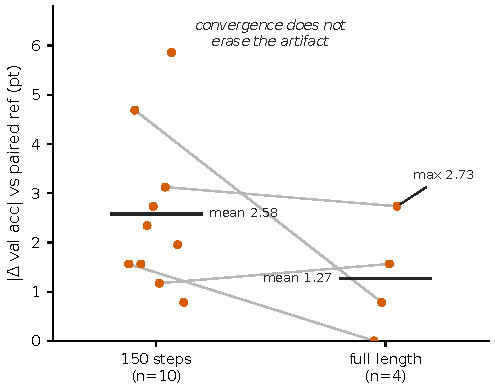
\includegraphics[width=3.3in]{figs/app_persistence.pdf}%
}{%
  \fbox{\parbox[c][2.97cm][c]{0.55\textwidth}{\centering
    Placeholder for \texttt{figs/app\_persistence.pdf}.}}%
}
\caption{Persistence of the probe displacement at convergence. Each dot is
one run's $|\Delta\,\text{val acc}|$ between the CUDA-probe arm and its
paired reference: ten 150-step pairs (mean $2.58$ points) versus four
full-length runs (mean $1.27$, maximum $2.73$); gray lines connect matched
(task, seed) pairs. This is the main text's claim that convergence shrinks
but does not erase the artifact.}
\label{fig:app-persistence}
\end{figure}

\subsection{PyTorch stream premises (\code{torch} 2.11.0)}

Proposition~1 treats PyTorch's global generators as streams in the sense
of Appendix~C.1. The four premises this requires are verified in source
and exercised empirically.

\begin{table}[tbp]
\centering
\footnotesize
\setlength{\tabcolsep}{5pt}
\begin{tabular}{@{}lL{7.2cm}L{6.6cm}@{}}
\toprule
 & Premise & Source citation \\
\midrule
P1 & Factory calls without \code{generator=} dispatch to the
process-global default generator & \code{ATen/core/Generator.h:159--168}
(default-generator dispatch) \\
P2 & \code{fork\_rng} saves the CPU state and the states of listed
devices on entry and restores them on exit &
\code{torch/random.py:209--217} \\
P3 & Draws through an explicit \code{torch.Generator} leave the global
defaults untouched & dispatch site as P1; exercised by the two explicit-generator
assertions of the check script \\
P4 & The CPU default and each CUDA device's default are distinct
generators & \code{torch/cuda/random.py:41} (per-device default
generators) \\
\bottomrule
\end{tabular}
\caption{The stream premises of Proposition~1, cited to \code{torch}
2.11.0 source. No premise remains unverified.}
\label{tab:premises}
\end{table}

\code{scripts/rng\_premise\_check.py} packages the premises as 13 boolean
assertions: three for global dispatch (P1: \code{rand},
\code{randint}, and \code{randperm} each advance the global CPU state),
three for fork-restore (P2: CPU state restored, CUDA state restored, and
the next draw after \code{fork\_rng} identical to the no-fork draw), two
for explicit-generator isolation (P3: global CPU and CUDA states
unchanged), and five for device separation (P4: distinct generator
objects; a CUDA draw advances CUDA state and leaves CPU state unchanged;
a CPU draw advances CPU state and leaves CUDA state unchanged). All 13
pass on the manifest stack (Appendix~E), exercising both the CPU and the
CUDA device. A semantic detail confirmed at source: \code{fork\_rng}
always forks the CPU stream, and its \code{devices} argument governs
accelerators only, so a probe isolated by \code{fork\_rng} is complete in
both CPU-only and CUDA execution.

\section{Proofs}
\label{sec:proofs}

\subsection{Setting: streams, cursors, probes}
\label{sec:setting}

Notation follows the main text: $\theta$ parameters, $\eta$ learning
rate, $\Delta$ signed paired difference, $m$ probe realizations, $n$
probe-split size, $s$ seed.

\paragraph{Deterministic execution (K).}
All paired experiments run under deterministic kernels (Appendix~D):
every operation's output is a fixed function of its inputs, so a run is a
deterministic function of its initial state and of the values it reads
from streams.

\paragraph{Streams as cursored sequences.}
A \emph{stream} is a shared stateful sequence with a monotone cursor: an
ordered value sequence $V = (v_1, v_2, \dots)$ and a cursor $c$, where
consuming $k$ items returns $v_c, \dots, v_{c+k-1}$ and advances
$c \mapsto c + k$; outside explicit restoration or reseeding,
only consumption moves $c$. Two families instantiate
this in training. (a) \emph{PRNG streams}: deterministic state machines
$(v_i, s_{i+1}) = f(s_i)$ with $s_1$ fixed by the seed, so $V$ is a
function of the seed: the process-global PyTorch CPU generator, each
per-device CUDA generator, the NumPy global state, and Python's
\code{random} (Table~\ref{tab:premises}). (b) \emph{Data cursors}: shared
iterators whose cursor is an epoch pointer over a data order. The breadth
is load-bearing: the official L2RW evaluation desynchronizes its
comparison by advancing a data cursor, consuming no PRNG draw at all
(Table~\ref{tab:classic}, row~1).

\paragraph{Training-visible state; probes.}
Write $X$ for the complete \emph{non-stream} training state: parameters,
buffers (including normalization statistics), gradients, optimizer and
scheduler state, modes, caches, and control state, including anything else
read by a later training operation. Stream sequences and cursors are separate
state, not part of $X$. Their read values are explicit inputs $z_n$ to an
aligned deterministic update $X_{n+1}=F_n(X_n,z_n)$. An
operation block interleaved with training is a \emph{probe} if (P-a) it
writes no non-stream training state $X$ and (P-b) interacts with training only
by possibly advancing stream cursors. An evaluation pass that updates
BatchNorm running statistics, or any block that steps the optimizer, is
not a probe; Corollary~\ref{cor:noop} therefore carries state purity of
the framework's internal machinery as an explicit rather than tacit
premise.

\subsection{Proposition 1: the pairing condition}

\begin{propositionx}[Pairing condition]

Let $X$ be the complete non-stream training state, with stream sequences
and cursors tracked separately. Consider deterministic executions of the
same training program, initially identical in both kinds of state, with
aligned updates $X_{n+1}=F_n(X_n,z_n)$. A probe leaves $X$ unchanged and can
affect training only through stream cursors. Then (i) identical training
reads imply bitwise-identical $X$ trajectories; disjoint probe streams or
complete fork--restore suffice. (ii) A probe advancing one stream by
$k\ge1$ shifts its subsequent training reads by $k$ only along an aligned,
equal-consumption prefix with no further differential advance, restoration,
or reseeding.
The first divergence is the first aligned operation with common input
state $x$ and $F_n(x,z)\ne F_n(x,z')$, not merely different intermediate
values. Later reconvergence is possible. A probe affecting only streams
never subsequently read by training is inert. (iii) Preserving reads is
sufficient, not necessary: distinct read values can induce the same state
update. No necessity or probability-one divergence claim is made.
\end{propositionx}

\begin{proof}
\textbf{(i)} Induct over aligned training operations. The initial $X$ states
are identical. Probes leave $X$ unchanged; equal $X_n$ and equal reads
$z_n$ give equal $F_n(X_n,z_n)$ by determinism, including the control state
needed to align the next operation. Disjoint streams or restoration of every
touched training stream preserve those reads. Thus $X$ trajectories and
deterministic evaluations using identical evaluation inputs coincide. This
does not claim equality of un-restored, training-irrelevant stream cursors.

\textbf{(ii)} Immediately after the probe, the affected cursor difference is
$k$. Equal subsequent consumption counts preserve that difference until a
further differential advance, restoration, or reseeding; hence reads at
$i_j$ are compared with reads at $i_j+k$ on this prefix. Starting from equal
$X$, equality persists exactly while the realized update outputs agree.
Consequently its first failure occurs at the first actual inequality
$F_n(x,z)\ne F_n(x,z')$. A changed mask or batch alone does not establish
this inequality. After divergence, neither aligned control flow nor equal
consumption counts are guaranteed. Non-injective later updates can map
different states to the same state, so reconvergence is not excluded.
If no affected stream is subsequently read by training, all training reads
are preserved and (i) applies.

\textbf{(iii)} Sufficiency is (i). Necessity fails even for a nonconstant
update: $F(x,z)=x+z^2$ gives identical updates at $z=1$ and $z=-1$.
Cancelled contributions, clipping, and rounding supply further many-to-one
maps. Dependence on a draw is not injectivity in that draw. No distributional
claim about these equalities is required for the repair's sufficient condition.
\end{proof}

\begin{lemma}[Coupling versus marginal estimands]
\label{lem:coupling-estimands}
Let $U\sim P$ be the random input to two deterministic endpoint maps
$Y_M,Y_B$, with the expectations below finite (and second moments finite
for the variance identity), and let $T$ be the stream-shift map in the probed arm. Define
$\tau=\mathbb E_P[Y_M(U)]-\mathbb E_P[Y_B(U)]$ and
$\widetilde\Delta=Y_M(TU)-Y_B(U)$. Then, without any invariance assumption,
\[
\mathbb E[\widetilde\Delta]-\tau
 =\mathbb E_P[Y_M(TU)]-\mathbb E_P[Y_M(U)],
\quad
\operatorname{Var}(\widetilde\Delta)
 =\operatorname{Var}(Y_M(TU))+\operatorname{Var}(Y_B(U))
 -2\operatorname{Cov}(Y_M(TU),Y_B(U)).
\]
If $T_\#P=P$, the first quantity is zero, but the covariance term need not
equal the intended paired covariance. For a data cursor, $T_\#P=P$ is not
automatic and no marginal-unbiasedness conclusion follows from stream
algebra alone. For a history-dependent intervention after a history
$\mathcal H_t=h$, the corresponding sufficient condition is preservation
of the \emph{conditional} future-input law: $(T_h)_\#P_h=P_h$ almost surely,
where $P_h=\mathcal L(U_{>t}\mid\mathcal H_t=h)$. This must hold for the
complete joint future input used by the continuation.
\end{lemma}

\begin{proof}
Expand the expectation and variance of $Y_M(TU)-Y_B(U)$ and subtract the
definition of $\tau$. Measure preservation gives
$\mathbb E_P[Y_M(TU)]=\mathbb E_P[Y_M(U)]$; the covariance identity is
otherwise unchanged. Apply the same identity to the deterministic continuation
at each fixed history under conditional preservation, then use iterated
expectation.
\end{proof}

\begin{remarkx}[The statistical reading, and what is measured]
For a PRNG stream the shifted tail starts from its advanced internal state.
This mechanical fact implies neither a fresh-seed trajectory law nor
independence, Gaussian residuals, or reduced endpoint covariance. Even under
an ideal i.i.d.\ future stream and a fixed history-measurable displacement,
the retained training state and history remain shared; conditional
measure preservation can preserve a continuation's marginal law without
making the paired continuations independent. Adaptive displacement requires
its own invariance check. Realized divergence and its onset are trace
measurements, not consequences of changed intermediate values alone.
Endpoint magnitude, sign, and covariance are empirical properties; none is
derived from cursor arithmetic.
\end{remarkx}

\subsection{Proposition 2: harvest size}

\begin{propositionx}[Harvest size]

For a finite vector of integrable paired gaps $D=(D_1,\ldots,D_m)$, let
$\mu_j=\mathbb ED_j$, $\bar\mu=m^{-1}\sum_j\mu_j$, and let $J$ be a fixed
tie-broken maximizer of $D_j$. For arbitrary means and dependence,
\[
\mathcal O:=\mathbb E[D_J-\mu_J]
\ge\max_j\mu_j-\mathbb E\mu_J\ge0,\qquad
\mathbb EH(D)=\mathbb E[\mu_J-\bar\mu]+\mathcal O,
\]
where $H(D)=\max_jD_j-m^{-1}\sum_jD_j$. The mean-selection term need not be
positive. Common additive components cancel from $H$.
If $D_j=a+C+\sigma Z_j$, with $\sigma\ge0$, integrable common $C$ and i.i.d.\ standard
normals $Z_j$, then $\mathbb EH=\mathcal O=c_m\sigma$ and
$c_m=\mathbb E\max_jZ_j$. Independence of $C$ from the $Z_j$ is unnecessary.
\end{propositionx}

\begin{proof}
Since $D_J=\max_jD_j$, $\mathbb ED_J\ge\max_j\mathbb ED_j$;
subtracting $\mathbb E\mu_J\le\max_j\mu_j$ proves the inequalities.
Adding and subtracting $\mu_J$ in $D_J-\bar D$ proves the decomposition.
For example, deterministic $D=(0,3,6)$ gives $H=3$ but $\mathcal O=0$:
uplift need not be noise optimism. In the Gaussian special case,
$H(D)=\sigma(\max_j Z_j-\bar Z)$ pathwise and all $\mu_j$ are equal, so
$\mathbb EH=\mathcal O=c_m\sigma$. The maximum density is
$m\varphi(x)\Phi(x)^{m-1}$, hence
\[
c_m=m\int_{-\infty}^{\infty}x\,\varphi(x)\,\Phi(x)^{m-1}\,dx.
\]
Numerical quadrature gives the constants in Table~\ref{tab:cm}, in
particular $c_6=1.2672$ and $c_7=1.3522$.
\end{proof}

\begin{remarkx}[Offsets, dependence, and the scale being estimated]
Let $P=I-\mathbf1\mathbf1^\top/m$ and let $\alpha$ be deterministic. Since
$H(x)=\max_j(Px)_j$ and the maximum changes by between the smallest and
largest added coordinate,
\[
\min_j(P\alpha)_j\le
\mathbb EH(\alpha+\varepsilon)-\mathbb EH(\varepsilon)
\le\max_j(P\alpha)_j.
\]
Thus offsets need not leave a Gaussian benchmark or its ratio unchanged.
For $m\ge2$ and a square-integrable vector $D$ with mean $\mu$ and covariance
$\Sigma$, the within-grid sample variance $S^2=\|PD\|^2/(m-1)$ satisfies
\[
\mathbb ES^2=
\frac{\|P\mu\|^2+\operatorname{tr}(P\Sigma)}{m-1}.
\]
Indeed $\mathbb E\|PD\|^2=\|P\mu\|^2+
\operatorname{tr}(P\Sigma P)$ and $P^2=P$. The spread therefore mixes
mean contrasts and stochastic contrasts; offsets do not guarantee a
particular change in a realized maximum or observed-to-predicted ratio.

For equal-mean equicorrelated Gaussian residuals
$\varepsilon_j=\sigma(\sqrt\rho Z_0+\sqrt{1-\rho}Z_j)$,
$0\le\rho<1$, the common factor cancels and
$\mathbb EH=c_m\sigma\sqrt{1-\rho}$. Here $\sigma$ is the \emph{marginal}
residual scale; a within-grid SD already estimates the contrast scale
$\sigma\sqrt{1-\rho}$. Multiplying it by another $\sqrt{1-\rho}$ would
double-correct correlation. Under equal means and i.i.d.\ normal residual
coordinates (or this common-factor extension),
$\mathbb ES=c_4(m)\sigma_{\rm contrast}$, where
\[
c_4(m)=\sqrt{\frac{2}{m-1}}\,
\frac{\Gamma(m/2)}{\Gamma((m-1)/2)}.
\]
This normal-theory correction (distinct from the maximum constant $c_4$)
does not generally hold with unequal means or arbitrary dependence.
Consequently $c_m\bar\sigma$ is an in-grid descriptive Gaussian benchmark,
not an independent prediction or a universal pricing law.
\end{remarkx}

\begin{remarkx}[Validation selection and held-out reporting]
Let $J$ maximize validation scores with fixed tie breaking and let integrable
$T_j$ be the corresponding test quantities, with $\mu_j^T=\mathbb ET_j$.
Candidate-specific centering gives the exact identity
\[
\mathcal O_T:=\mathbb E[T_J-\mu_J^T]
=\sum_{j=1}^m\operatorname{Cov}(\mathbf1\{J=j\},T_j).
\]
Expand $T_J$ with selection indicators to prove the identity. Its sign is
unrestricted: positive validation--test Pearson correlation does not fix
these selection-indicator covariances. For a finite counterexample, take
$x$ uniform on $(-2,-1,1,2)$, validation scores $(x,-x)$, and test scores
$(t,-t)$ with respective $t=(-10,15,-15,10)$. Both candidate correlations
are positive, but all test means vanish and $\mathcal O_T=-2.5$.
An observed selected test delta from a common baseline is not this optimism
unless the same candidate-specific mean reference is used. Stronger transfer
models may yield positive benchmarks; correlation alone is not such a model.
\end{remarkx}
\begin{table}[tbp]
\centering
\small
\begin{tabular}{@{}lcccccc@{}}
\toprule
$m$ & 2 & 3 & 4 & 5 & 6 & 7 \\
\midrule
$c_m$ (exact) & 0.5642 & 0.8463 & 1.0294 & 1.1630 & 1.2672 & 1.3522 \\
$\sqrt{2\ln m}$ & 1.1774 & 1.4823 & 1.6651 & 1.7941 & 1.8930 & 1.9728 \\
overshoot & $+108.7\%$ & $+75.2\%$ & $+61.8\%$ & $+54.3\%$ & $+49.4\%$ &
$+45.9\%$ \\
\bottomrule
\end{tabular}
\caption{The asymptotic $\sqrt{2 \ln m}$ is unusable at the $m$ of real
reporting practices: exact expected maxima of $m$ standard normals
(quadrature of the expression in the proof) against the leading-order
asymptotic and its relative overshoot.}
\label{tab:cm}
\end{table}

\begin{remarkx}[Why not $\sqrt{2\ln m}$]
Extreme-value asymptotics give
\[
c_m = \sqrt{2\ln m}
\;-\; \frac{\ln \ln m + \ln 4\pi}{2\sqrt{2\ln m}}
\;+\; \frac{\gamma}{\sqrt{2\ln m}} \;+\; o\bigl((\ln m)^{-1/2}\bigr),
\]
with $\gamma$ the Euler--Mascheroni constant. The leading term alone
overshoots the exact constant by $+49.4\%$ at $m = 6$ and $+45.9\%$ at
$m = 7$ (Table~\ref{tab:cm}), the negative second-order term staying
non-negligible until $\ln \ln m \gg 1$. A prediction built on
$\sqrt{2 \ln m}$ would have overshot the measurement by half, so the data
are tested against the exact constants and the asymptotic form is kept
only as growth-law language.
\end{remarkx}

\begin{remarkx}[Common components and shared baselines]
The invariance clause is what makes the statistic measurable here: all
placements within a seed share one baseline run, so the baseline's
realization enters every paired gap $\Delta_j$ as a common component and
cancels exactly in max-minus-mean, as does any common probe main effect.
What survives is the placement contrast, which may contain unequal means
as well as noise. Proposition~\ref{prop:pairing}(ii) does not specify its law.
\end{remarkx}

\begin{remarkx}[Model premises and reviewer-requested sensitivity]
Independence and approximate normality are modeling premises, not theorems.
The nested growth curve reuses the placement cells used to estimate
$\bar\sigma$, so it is an in-grid shape check, not independent prediction.
Exact quadrature gives the descriptive comparison $\RevHarvest$ points of
uplift versus $c_6\bar\sigma=\RevPrediction$; the normal-specific
$c_4(m)$ correction gives $\RevCorrectedPrediction$. The uncorrected ratios
for shortened, realistic-evaluation, full-best and full-final endpoints are
$0.9734$, $1.1463$, $1.0075$, $1.0034$; the corrected ratios are
$0.9262$, $1.0775$, $0.9282$, $0.9245$. Best and final share three seeds
and are not independent replications.

The reviewer-requested bootstrap jointly resamples each complete seed row
in numerator and denominator, enumerating all $5^5=3{,}125$ or $3^3=27$
ordered samples. Corrected percentile intervals are respectively
$[0.7003,1.1155]$, $[0.8945,1.2009]$, $[0.8665,0.9776]$ and
$[0.6611,1.2452]$. The full-best interval excludes one, but these discrete
three-seed resamples do not establish calibrated coverage or reliable model
rejection. Unequal placement means and contrast covariance can enter the
fitted scale: the empirical placement covariance and row-centered contrast
covariance have rank four with five seeds and rank two with three seeds,
and do not validate an unrestricted covariance model.

The original constant-only Gaussian/$t_3$ curves use $200{,}000$ Monte Carlo
draws; their reproducibility does not establish iid residuals. The new
full-procedure sensitivity instead generates $100{,}000$ complete matrices
under normal and variance-matched $t_3$ models, re-estimating every SD and
the ratio of means in each replicate (fixed seed $20260908$). At $5\times6$,
the normal-corrected ratio has means $0.9997$ and $1.0177$ and respective
sampling-reference intervals $[0.8087,1.1979]$ and $[0.7251,1.3014]$;
at $3\times4$ the means are $1.0001$ and $1.0008$. Using observed
$s_s/c_4(m)$ as fixed seed-specific scales gives similarly overlapping
references. Thus constant-only $t_3$ underprediction does not discriminate
the residual distributions once scale estimation is included. The normal
$c_4(m)$ multiplier is part of the same statistic in both simulations,
not a valid $t_3$ unbiased-scale correction. These are simulation
sensitivities, not additional training evidence.
\end{remarkx}

\begin{remarkx}[The cross-seed prediction, and what it refutes]
The historical cross-seed implementations use different scales:
\code{scripts/prop2\_fit.py} flattens the remaining rows before calculating one SD,
whereas \code{figs/make\_fig\_r1\_crossseed.py} averages their within-row SDs.
The former mixes between-seed means into the scale; both are reported in
the canonical reanalysis. For the latter, predicting the fifth seed's
max-minus-mean as $c_6\bar\sigma$ \emph{fails at the individual-seed level}.
Predicted versus observed
(points): $3.95/3.00$, $4.38/2.71$, $3.87/5.39$, $4.71/1.63$, $3.70/7.32$:
mean absolute error $2.17$, $54\%$ of the $4.01$ being predicted, with the two
series \emph{anti}-correlated ($r=-0.8672$); mean signed error is $+0.11$.
The flattened-row alternative has MAE $2.2441$ and $r=-0.9683$; the
$c_4(m)$-corrected within-row alternative has MAE $2.2210$.
Mean-other-SD predictions are affine decreasing functions of held-out SD,
so their correlation with harvest is the negative of the \emph{observed}
SD--harvest correlation, not necessarily negative in every population or
dataset. Substituting each seed's own SD reduces MAE to $0.8256$, but uses
the same outcomes as the measured harvest and is not a held-out validation.
These results document failed seed-level scale transport; they neither
independently validate nor isolate the Gaussian constant as the sole correct
part of the model. We make no per-run prediction from the aggregate fit.
\end{remarkx}


\begin{remarkx}[Instantiation constants and statistic definitions]
$m$ is fixed by design, not fitted. The multi-seed campaign uses $m = 6$
placements per seed ($c_6$; numbers above). The single-seed official-code
demonstration uses $m = 7$ ($c_7$): its selection max-minus-mean over the
8-realization set (7 placements plus the no-probe run) is $+2.88$
($32.60 - 29.72$), a single-seed realized value rather than a mean, and
$+3.06$ over the 7 placements alone (an earlier 6-placement mid-campaign
figure of $+3.24$ is superseded). In the same set the honest average
placement effect is $-1.44$ and the worst single placement $-8.68$
(reproduced exactly at Appendix~D's floor resolution under a different
concurrency condition): the probe hurts on average. The selected maximum's
uplift over the placement average is not an identified noise-only gain.
The multi-seed grid these
constants are read off is Figure~\ref{fig:app-harvest-heatmap}.
\end{remarkx}

% Supplementary figure: the multi-seed harvest grid.
\begin{figure}[t]
\centering
\IfFileExists{figs/app_harvest_heatmap.pdf}{%
  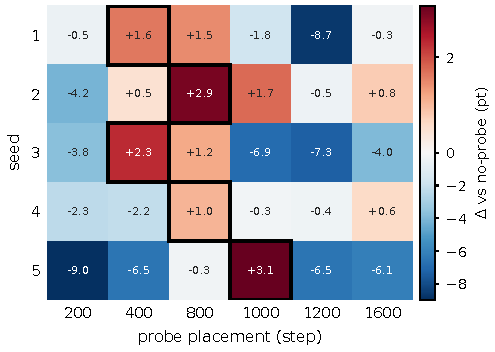
\includegraphics[width=3.3in]{figs/app_harvest_heatmap.pdf}%
}{%
  \fbox{\parbox[c][2.97cm][c]{0.55\textwidth}{\centering
    Placeholder for \texttt{figs/app\_harvest\_heatmap.pdf}.}}%
}
\caption{The harvest grid behind the Proposition~\ref{prop:harvest} fit:
paired deltas (points) for 5 seeds $\times$ 6 probe placements, diverging
scale centered at $0$, per-seed maximum outlined. The grid spans $-8.98$
to $+3.08$ points with honest mean $-1.82$; the outlined maxima ($+1.62$,
$+2.92$, $+2.30$, $+1.04$, $+3.08$) are what per-seed selection reports,
and the $-8.68$ cell (seed 1, step 1200) is the floor-verified outlier of
Table~\ref{tab:floors}. The maxima land on three different placements. A
legacy placement test gives $p=0.049$ under within-seed permutation,
conditional on exchanging fixed training positions being a valid null.
The general part of Proposition~\ref{prop:harvest}
allows unequal means, but its Gaussian special case does not absorb them:
$\sigma$ is estimated as within-seed spread \emph{across} placements and mixes
offset and noise contrasts, without a guaranteed matching change in the
observed maximum. In simulation, treating the observed column means
as real offsets moves the \emph{expected} observed-to-predicted ratio from
$1.00$ to $1.04$ (a sensitivity check, not one of the campaign ratios of
Figure~\ref{fig:ratios}), and the observed harvest sits at the $53$rd
percentile of the null in which no placement effect exists at all.}
\label{fig:app-harvest-heatmap}
\end{figure}

\subsection{Proposition 3: meta-signal scale}

\begin{proposition}[Meta-signal scale]
\label{prop:deadmeta}
For a single SGD virtual step
$\theta'(w) = \theta - \eta \nabla_\theta \sum_i w_i \ell_i(\theta)$ and
a meta-objective $L_{\mathrm{meta}}(\theta')$ with no direct
$w$-dependence,
$\partial L_{\mathrm{meta}} / \partial w_i =
-\eta\, \langle \nabla L_{\mathrm{meta}}(\theta'),
\nabla \ell_i(\theta) \rangle$ exactly; the meta-signal is $O(\eta)$ for
bounded gradients, while any $\eta$-independent term competing for the
same weights is unmoved. If, in addition, $\nabla L_{\mathrm{meta}}$ is
locally Lipschitz near fixed $\theta$ and the weighted update direction is uniformly
bounded as $\eta\to0$ (in particular, for fixed $w$), the direction
field has an $O(\eta)$ perturbation within that neighborhood. For a
nonzero limiting direction and a nonzero normalization denominator, a
post-map $w=N(\mathrm{signal})$ removes the explicit multiplicative $\eta$
scale iff $N$ is positively homogeneous of degree zero; it does not remove
direction changes, and the zero-direction case is outside this claim.
\end{proposition}

\begin{proof}
The virtual step is affine in $w$ with a $w$-independent Jacobian:
$\theta'(w) = \theta - \eta \sum_j w_j \nabla_\theta \ell_j(\theta)$,
where $\theta$ and the per-example gradients
$\nabla_\theta \ell_j(\theta)$ are evaluated at the unperturbed point and
do not depend on $w$; hence
$\partial \theta' / \partial w_i = -\eta\, \nabla_\theta \ell_i(\theta)$
exactly. Because $L_{\mathrm{meta}}$ has no direct $w$-dependence, the
chain rule gives, with no expansion in $\eta$,
\[
\frac{\partial L_{\mathrm{meta}}(\theta'(w))}{\partial w_i}
\;=\; \Bigl\langle \nabla_{\theta'} L_{\mathrm{meta}}(\theta'),\,
\frac{\partial \theta'}{\partial w_i} \Bigr\rangle
\;=\; -\eta\, \bigl\langle \nabla L_{\mathrm{meta}}(\theta'),\,
\nabla \ell_i(\theta) \bigr\rangle .
\]
Both stated conditions are load-bearing. Multiple inner steps or an
adaptive inner update are outside this identity: their exact Jacobians and
leading-order scales require separate derivation. A direct $w$-dependence
of the meta-objective adds an
$\eta$-free term to $\partial L_{\mathrm{meta}} / \partial w_i$, exactly
the competition mode the proposition prices. For scale,
$|\partial L_{\mathrm{meta}} / \partial w_i| \le
\eta\, \lVert \nabla L_{\mathrm{meta}}(\theta') \rVert\,
\lVert \nabla \ell_i(\theta) \rVert$, so with gradients bounded on the
visited set the meta-signal is $O(\eta)$, an upper envelope rather than
a guaranteed magnitude, since the inner product can vanish, which is why
the statement is $O(\eta)$ and not $\Theta(\eta)$. An input to the same
consumer carrying no factor of $\eta$ is unmoved as $\eta \to 0$; what that
costs a controller in practice is the subject of
Section~\ref{sec:deadmeta-taxonomy}.

\emph{Normalization escape.} Write the signal field as
$g_\eta = -\eta\, h_\eta$ with
$h_{\eta,i} = \langle \nabla L_{\mathrm{meta}}(\theta - \eta G w),\,
\nabla \ell_i(\theta) \rangle$ and
$Gw = \sum_j w_j \nabla \ell_j(\theta)$; then, for fixed $\theta$,
uniformly bounded $Gw$ and $\nabla L_{\mathrm{meta}}$ locally Lipschitz near $\theta$,
$h_\eta = h_0 + O(\eta)$, so the $\eta$-dependence factors into an exact
multiplicative scale and an $O(\eta)$ perturbation of the direction. Say a
post-map $N$ \emph{removes the scale} if $N(\eta h) = N(h)$ for every
signal $h$ in its domain and every $\eta > 0$; we prove this holds iff $N$
is positively homogeneous of degree zero, i.e.\ $N(c\,x) = N(x)$ for all
$c > 0$ and $x$ in the domain.
($\Leftarrow$) $N(g_\eta) = N\bigl(\eta \cdot (-h_\eta)\bigr) =
N(-h_\eta)$: the scale is removed exactly, and residual $\eta$-dependence
enters only through the $O(\eta)$ rotation of the direction.
($\Rightarrow$) Fix $x$ in the domain and $c > 0$; apply the removal
property with $h = x$ at $\eta = c$ and at $\eta = 1$:
$N(cx) = N(x)$.
\end{proof}

\begin{remarkx}[Sum-to-one is not the property]
$\mathrm{softmax}(c\,g)$ tends to the uniform vector as $c \to 0^{+}$
for every non-constant $g$: softmax sums to one, is invariant to additive
shifts, and is not positively homogeneous of degree zero. Fed an
$\eta$-scaled signal, a softmax-normalized controller's weight contrasts
vanish as $\eta\to0$, but need not be zero at finite $\eta$.
What rescues the rectify-then-normalize map used by
L2RW is homogeneity:
$N(g) = \mathrm{ReLU}(g) / \langle \mathbf{1}, \mathrm{ReLU}(g) \rangle$
is a ratio of two positively 1-homogeneous maps, hence 0-homogeneous
wherever the denominator is nonzero.
\end{remarkx}

\begin{remarkx}[The zero-guard is load-bearing]
Both audited L2RW implementations guard the normalization at exactly zero:
the TF release increments the denominator only when it equals $0.0$
(\code{reweight.py:150--153}), and the PyTorch notebook branches on
\code{norm\_c != 0}, so the guard fires only when the rectified signal
is exactly zero, i.e.\ when no example carries positive signal, and the
escape is intact for every nonzero signal. A threshold variant (normalize only when
$\sum_i \mathrm{ReLU}(g_i) > \delta$ for fixed $\delta > 0$) bypasses
scale cancellation whenever the rectified sum is at or below $\delta$:
the raw $\eta$-scaled weights pass through. This branch does not itself
imply zero action or establish that every batch crosses the threshold.
\end{remarkx}

% Supplementary figure: signal-vs-update decoupling (Prop. 3 instantiated).
\begin{figure}[t]
\centering
\IfFileExists{figs/app_f1_decoupling.pdf}{%
  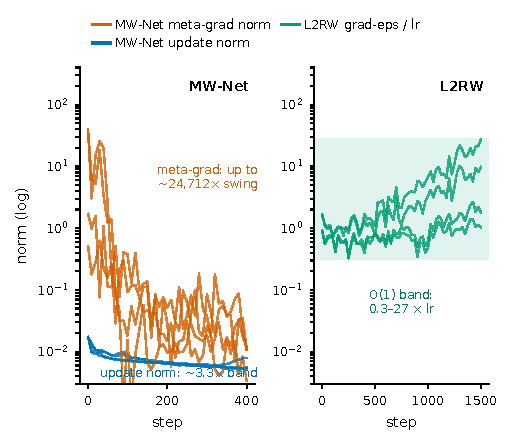
\includegraphics[width=3.3in]{figs/app_f1_decoupling.pdf}%
}{%
  \fbox{\parbox[c][2.97cm][c]{0.55\textwidth}{\centering
    Placeholder for \texttt{figs/app\_f1\_decoupling.pdf}.}}%
}
\caption{Signal-versus-update decoupling in the two re-executed
meta-reweighting systems (four runs each: noise $\{0, 0.4\} \times$ seeds
$\{1, 2\}$). Left: Meta-Weight-Net's raw meta-gradient norm (vermillion)
decays $150\times$--$3{,}700\times$ from first to last measurement across
the four runs, and its full within-run
$\max/\min$ swing reaches ${\sim}24{,}700\times$, while the induced v-net
update norm (blue) stays inside a $3.3\times$ band throughout. Right:
L2RW's raw meta-gradient divided by the learning rate lies between $0.32$
and $27$ (shaded), consistent with raw $O(\eta)$ scaling. The separate
rectify-then-normalize map removes the explicit scale by
0-homogeneity (Proposition~\ref{prop:deadmeta}); applied weights are not plotted.}
\label{fig:app-f1-decoupling}
\end{figure}

\subsection{The dead-meta-gradient taxonomy (a second, appendix-scoped
diagnosis)}
\label{sec:deadmeta-taxonomy}

This diagnosis is deliberately appendix-scoped. The main text carries the
paper's contribution: a condition, a prevalence audit, byte-level witnesses, a
harvest law, and a repair. What follows is a second, narrower
diagnosis of the same method family, established analytically and instrumented
in three systems (Figure~\ref{fig:app-f1-decoupling}) rather than audited at
scale, and reported because it lands on the same victims.

Proposition~\ref{prop:deadmeta}'s $O(\eta)$ scale can become negligible in
\emph{competition}: the relevant magnitude ratio compares the $\eta$-scaled
signal with whatever else reaches the same weights. An $\eta$-independent
input of comparable or larger size (a regularizer, a fixed-scale update)
can dominate a signal scaled by $\eta\approx10^{-5}$--$10^{-3}$, but this
does not imply exactly zero controller action. The outcome depends on the
consumer and the learning-rate schedule, not merely on the presence of a
competing term. Three named escapes can mitigate this sensitivity: a degree-0-homogeneous weight map
cancels the explicit multiplicative scale, while an independent adaptive
optimizer can reduce (but, with the usual $\epsilon>0$, does not exactly
remove) sensitivity to gradient magnitude. A signal that is
$\eta$-independent by construction (a real validation-metric difference
between materialized candidate models, the choice our constructive endpoint
makes) sidesteps the competition entirely (Table~\ref{tab:f1}). The dead
regime is not hypothetical: our own predecessor system was the specimen, its
signal ${\sim}10^{-6}$ against a ${\sim}10^{-4}$ regularizer, every learned
amplitude pinned at initialization and its ``filtering'' map identically the
identity for entire runs.

\begin{table}[tbp]
\centering
\small
\begin{tabular}{@{}p{0.17\columnwidth}p{0.33\columnwidth}p{0.36\columnwidth}@{}}
\toprule
Class & Signal path & In-system evidence \\
\midrule
Dead &
lr-scaled virtual step; consumer shares parameters with an
$\eta$-independent regularizer &
in-house predecessor: signal ${\sim}10^{-6}$ vs.\ own regularizer
${\sim}10^{-4}$; weights pinned ($\pm 0.5\%$); filtered/raw
$\equiv 1.0000$ \\
\addlinespace
Rescued by construction &
virtual step, then rectify-and-normalize weight map (degree-0 homogeneous) &
L2RW PyTorch reimplementation, driven unmodified: lr-normalized raw gradient
$\lVert g_\epsilon \rVert / \eta = O(1)$ throughout training (0.3--27
across four runs) \\
\addlinespace
Decoupled by construction &
true meta-gradient consumed by an independent Adam optimizer &
MW-Net official, driven unmodified: update norm holds a ${\sim}3.3\times$
band while the raw meta-gradient swings $150\times$--$3{,}700\times$
first-to-last over the same window across the four runs \\
\bottomrule
\end{tabular}
\caption{A structural taxonomy of meta-controller signal paths, classified by
the signal's route to its consumer. The claim is signal \emph{scale reaching
the consumer}, not end-task efficacy; per-row evidence is in native units
because raw magnitudes are confounded by $\eta$, phase, and norm convention.}
\label{tab:f1}
\end{table}

The design rule is to check the signal's scale at its consumer: an
$\eta$-independent quantity or a scale-invariant map can avoid explicit
lr-scale competition, while adaptive optimization can mitigate it. An
lr-scaled signal may become negligible relative to a fixed-scale competing
term as the learning rate decays; exact inactivity requires additional
consumer behavior or measurement. This is why the two diagnoses fall on the
same victims: the virtual-step probe that makes a controller's signal scale
suspect is also the most RNG-hungry pattern in our audit, so the method family
that most needs trustworthy paired evaluation is the one whose default
implementation most reliably destroys it.

We state the scope plainly, because the analysis is more general than the
measurement. Proposition~\ref{prop:deadmeta} fixes the signal's scale exactly
and for every method of this form; whether that scale is \emph{fatal} is a
question about a magnitude ratio, and we measured that ratio in three
instrumented systems rather than mapping it across the method family, across
learning-rate regimes, or across competing-term sizes. This is therefore a
theoretically grounded failure mode illustrated in three systems, not a generic
fate of virtual-step controllers. The proportions matter and we state them:
exactly one of the three is dead, and it is our own predecessor; both
\emph{released} systems we instrumented escape, L2RW by a
degree-0-homogeneous weight map and Meta-Weight-Net by an independent adaptive
optimizer. Nothing here claims that any published method fails at its end task,
and those two escapes are evidence that the pattern is avoidable. How often it
is avoided in the wild is not something three instrumented systems can say.

\subsection{Corollary: the certified no-op}

\begin{corollaryx}[Certified no-op]

Under the deterministic pairing protocol of Appendix~D and state-pure,
stream-isolated candidate maintenance, champion $=$ raw implies that the
served model state (parameters and buffers) is bitwise identical to the
paired baseline endpoint, and hence every deterministic reported metric
delta is exactly zero. Conversely, a bitwise baseline identity implies
champion $=$ raw only under the additional, checked premise that every
non-raw candidate differs from raw in at least one parameter bit. Candidate
collisions (for example an EMA landing exactly on the endpoint) are not
excluded by training having moved and must be treated as exact-collision
events rather than assumed impossible.
\end{corollaryx}

\begin{proof}
State and stream isolation preserves every training consumption, so
Proposition~\ref{prop:pairing}(i) gives
$\theta_M^{\rm raw}\equiv\theta_B$ for the full endpoint state. If
champion $=$ raw, the served state equals $\theta_M^{\rm raw}$ and hence
equals $\theta_B$; deterministic evaluation on a fixed set then gives exact
metric equality. For the converse, if the served state equals $\theta_B$ and
champion is non-raw, the checked distinct-candidate premise says that served
state differs from $\theta_M^{\rm raw}\equiv\theta_B$, a contradiction.
\end{proof}
\begin{remarkx}[Resolution, and the falsification lever]
The ($\Leftarrow$) direction is a statement about weight-level identity.
At metric resolution it is not invertible (two different models can
collide at $1/n$ accuracy resolution), so the certificate is
operational rather than metric-inferred: the controller logs its
champion. A certificate requires the state-purity and isolation premises,
not just a raw champion and a zero metric floor. A nonzero delta in a
champion-raw cell falsifies the premise conjunction but does not uniquely
identify stream displacement: hidden state mutation or an untested
nondeterministic path can also account for it. Across the evaluated campaigns
every champion-raw cell reported exactly zero (18/18 tuned,
Table~\ref{tab:certreg}; 6/6 under-tuned canaries); the count includes metric-only cells without an independent floor, so it is not a bitwise certificate. The two other exact
zeros are EMA holdout ties logged as promotions rather than certificates.
\end{remarkx}

\begin{table}[tbp]
\centering
\footnotesize
\setlength{\tabcolsep}{5pt}
\begin{tabular}{@{}L{5.5cm}ccc@{}}
\toprule
Tuned regime & Guard $\Delta$ & Exact zeros & LAWA \\
\midrule
NLP, linear decay (3 tasks $\times$ 3 seeds) & \textbf{0.00} & 9/9 &
$-1.44$ (6/9 neg) \\
Vision SGD, clean & \textbf{0.00} & 5/5 & $-0.11$ (4/5 neg) \\
Vision SGD, noise30 & \textbf{0.00} & 5/5 & $-1.16$ (5/5 neg) \\
\bottomrule
\end{tabular}
\caption{Observational guard registry, not a count of state-level
certificates. The reported delta is zero in all 19 cells and champion $=$
raw in 18. The eight NLP raw-champion cells were historically described as
hash-verified, but the recovered per-cell logs contain no independently
checkable weight hashes and have no repeat floors; they are excluded from
certificate counts. The ten vision cells have metric-level evidence only
(Figure~\ref{fig:ledger}); the nineteenth is an exact
EMA--baseline holdout tie logged as a promotion, while unguarded
fixed-window averaging (LAWA) nets harm on the identical protocol.}
\label{tab:certreg}
\end{table}

\subsection{Lemma: margin calibration under paired probe noise}

This auxiliary selection analysis is not needed for the pairing condition
or the no-op implication. We retain its proof and the candidate-comparison
figures to document the guarded endpoint separately from the main diagnosis.

\begin{lemma}[Margin calibration]
\label{lem:margin}
At a selection event, a candidate is scored against raw on the same probe
split. Let $D_i\in\{-1,0,1\}$ be the paired correctness difference,
$D=\sum_i\mathbf 1\{D_i\ne0\}$ the discordant count, and
$W=\sum_i\mathbf 1\{D_i=1\}$ the candidate-win count. Assume only that the
probe examples are i.i.d. for this fixed candidate. If its population paired
effect satisfies $\Delta=\Pr(D_i=1)-\Pr(D_i=-1)\le0$, then conditional on
$D=d$, $W\sim\operatorname{Bin}(d,\pi)$ with $\pi\le1/2$. Consequently, any
promotion threshold $w_\alpha(d)$ satisfying
\[
\Pr\{\operatorname{Bin}(d,1/2)\ge w_\alpha(d)\}\le\alpha
\]
has conditional and unconditional false-promotion probability at most
$\alpha$. For $C$ candidates at one event, use $\alpha/C$; for $K$ planned
events, allocate levels $\alpha_{e,c}$ with $\sum_{e,c}\alpha_{e,c}\le\alpha$.
This requires a valid marginal test for every indexed comparison: for
example, all compared model pairs fixed independently of the reused probe,
or fresh i.i.d. probe examples independent of each adaptively chosen pair
conditional on its past. No independence among such valid tests is needed
for the union bound. Alpha allocation alone cannot make adaptively reused
probe data valid, even for a finite number of comparisons.
\end{lemma}

\begin{proof}
Write $q=\Pr(D_i=1)$ and $r=\Pr(D_i=-1)$. Conditional on discordance,
the win probability is $\pi=q/(q+r)$ (unless $q+r=0$), and
$\Delta=q-r\le0$ implies $\pi\le1/2$. The binomial tail is monotone in its
success probability, so the stated threshold is conservative conditionally
on every $D=d$; averaging over $D$ proves the unconditional bound. Bonferroni
gives the displayed allocations without any cross-event independence.
\end{proof}
\begin{remarkx}[Scope of the margin result]
The conditional rule avoids a guessed variance reduction or a population
accuracy replaced by its same-probe estimate. It is a prospective calibration
option, not a retrospective error guarantee for the historical fixed-margin
campaigns. State-pure RNG isolation does not make an adaptively reused
validation set statistically fresh. The no-op corollary is a separate
pathwise statement and does not require this false-promotion guarantee.
\end{remarkx}

\begin{remarkx}[Small $n$, conservatism, and the realized error profile]
For a small discordant count $D$, normal-tail calibration can be inaccurate;
the conditional binomial test handles that discreteness exactly under its
fixed-pair sampling premise. The guard inherits the conservative
side by design: strict inequality plus tie-to-raw resolution biases errors
toward keeping raw, whose cost is exactly zero by
Corollary~\ref{cor:noop} under its premises. The historical campaign record
has no negative observed holdout deltas in 19 tuned cells (one exact tie was
promoted), and one realized selection loss in 35
under-tuned cells ($-3.12$; the candidate cleared its margin on the probe and
failed to generalize to the holdout, the residual risk a probe margin
cannot price, reported rather than averaged away). What the guard pays out
where it does act, against LAWA and against an unconditional always-EMA
policy, is Figures~\ref{fig:app-payout-bars} and~\ref{fig:app-symmetry}; the
cell-by-cell record and its largest single rescue are
Figures~\ref{fig:app-nlp-strip} and~\ref{fig:app-cola-case}, and the
participation-ratio detector that gates the candidates is
Figure~\ref{fig:app-detector-grid}.
\end{remarkx}

\section{The Deterministic Pairing Protocol and the Repeat-Floor
Registry}
\label{sec:protocol}

\subsection{Protocol}

\begin{enumerate}\itemsep2pt
\item \textbf{Deterministic kernels.} Every paired run uses deterministic kernels:
\begin{itemize}\itemsep1pt
\item \code{torch.use\_deterministic\_algorithms(True)} (which also
constrains cuDNN to deterministic algorithms; with \code{warn\_only=True} in
the DivideMix and BHN witnesses);
\item \code{CUBLAS\_WORKSPACE\_CONFIG=":4096:8"}, exported before CUDA
context creation, as cuBLAS determinism requires (the NLP harness: see
below).
\end{itemize}
The nanoGPT campaign additionally sets
\code{torch.backends.cuda.matmul.allow\_tf32 = False} and
\code{torch.backends.cudnn.allow\_tf32 = False}; the other campaigns leave
TF32 at the PyTorch defaults, and their per-path repeat floors (item~3) are
measured under those settings.
The NLP harness reaches deterministic execution through \code{transformers}'
\code{enable\_full\_determinism(seed)}, which sets
\code{CUBLAS\_WORKSPACE\_CONFIG=":16:8"} itself. Proposition~1 is stated under
deterministic execution, and the second layer is real: in the under-tuned
CIFAR-100 protocol, same-seed cross-arm bifurcation from nondeterministic
kernels alone reached 11.7 points (Figure~\ref{fig:app-kernel-noise}).
\item \textbf{Stream isolation for every internal consumer.} Every monitor
statistic and controller probe executes inside \code{torch.random.fork\_rng}
with the active accelerator listed (\code{devices=[device]} under CUDA,
\code{devices=[]} on CPU), which forks
the CPU stream unconditionally and the listed device streams (Appendix~B.2):
the fork-restore discipline of Proposition~\ref{prop:pairing}(i). Probes are
state-pure in the sense of Appendix~C.1: eval-mode forwards, no optimizer
interaction, candidates kept as CPU-resident snapshots.
\item \textbf{The repeat-floor procedure.} Each materially distinct execution
path receives its own within-path repeat: both arms are rerun when their
kernel, control flow, precision, stochastic consumer, or probe differs,
unless a shared path has been explicitly established. The
\emph{repeat-floor} is the largest difference observed at the resolution of
the claim: metric-exact supports only a metric claim, weight-exact supports
only the recorded parameters and buffers, and full-state or trajectory
claims require hashes of the corresponding optimizer, scheduler/scaler,
controller, RNG/cursor, and checkpoint states. A zero floor is evidence on
the tested path, not a universal determinism proof; a nonzero floor voids the
family's paired reading. The floor converts ``we set seeds'' from a hope into
a measurement.
\item \textbf{Atomic result writes and completeness audits.} Campaign outputs
are written to a temporary file and moved into place by atomic rename
(\code{tmp} $+$ \code{os.replace}), so an interrupted run cannot leave a
truncated file that aggregation would read as complete; line counts audit
completeness (30/30 run files, zero holes, under-tuned NLP campaign).
\item \textbf{Regime hygiene.} Deltas from non-deterministic legacy campaigns
never enter deterministic tables, and where a legacy figure did not survive
re-measurement only the deterministic value is reported (CIFAR-100 clean:
legacy $+8.59$ withheld, deterministic re-measurement $+4.86$).
\end{enumerate}

% Supplementary figure: kernel nondeterminism (second layer).
\begin{figure}[t]
\centering
\IfFileExists{figs/app_kernel_noise.pdf}{%
  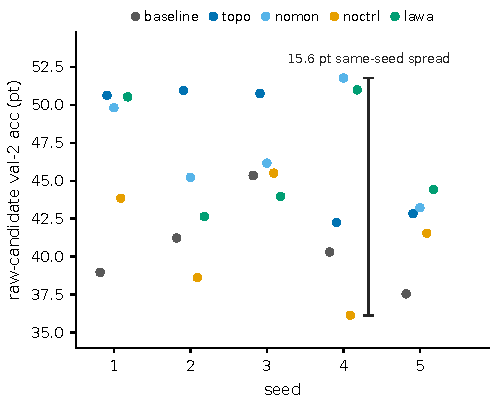
\includegraphics[width=3.3in]{figs/app_kernel_noise.pdf}%
}{%
  \fbox{\parbox[c][2.97cm][c]{0.55\textwidth}{\centering
    Placeholder for \texttt{figs/app\_kernel\_noise.pdf}.}}%
}
\caption{Kernel nondeterminism alone breaks same-seed pairing (legacy
non-deterministic CIFAR-100 stratified campaign, clean labels): every arm
trains the same recipe from the same seed, yet the raw candidates spread
by $6.8$--$15.6$ points within a seed. Dots are the five arms per seed;
the bracket marks the widest five-arm $\max{-}\min$ spread ($15.6$ points,
seed 4). The main text's $11.7$-point figure is the pairwise
topo-versus-baseline gap on seed 1 ($50.62$ vs.\ $38.96$), a two-arm
special case of the same bifurcation; the deterministic protocol above
eliminates it (repeat floors exactly $0$).}
\label{fig:app-kernel-noise}
\end{figure}

\subsection{Per-campaign repeat-floor registry}

\begin{table}[tbp]
\centering
\footnotesize
\setlength{\tabcolsep}{5pt}
\begin{tabular}{@{}L{4.4cm}L{7.6cm}L{3.2cm}@{}}
\toprule
Experiment family & Floor evidence & Comparison resolution \\
\midrule
HuggingFace probe experiments (RoBERTa-base; RTE, MRPC; five-arm,
ten-pair effect size, full-length) &
16 floor files across the campaigns, all exactly $0.0$: each repeat arm
verified bitwise identical to its reference &
weight-level $\max|\Delta W|$ \\
\addlinespace
NLP tuned, gate B (RTE/MRPC/CoLA $\times$ 3 seeds, linear decay) &
\emph{no independent rerun}: 8/9 cells champion $=$ raw with $\Delta$
exactly $0.00$;
the ninth (MRPC seed~2) an exact EMA--baseline holdout tie at
$\Delta = 0.00$ &
metric-exact; not a rerun \\
\addlinespace
NLP under-tuned (3 tasks $\times$ 5 seeds) &
30/30 run files complete (line-count audit, zero holes); \emph{no
independent rerun}: the 6 champion-raw cells are observations only, all at
$\Delta$ exactly $0.00$
(a seventh exact zero is an EMA-champion holdout tie) &
final metric, exact; not a rerun \\
\addlinespace
Vision tuned, deterministic (CIFAR-10, SGD cosine $+$ augmentation;
clean and noise30) &
repeat floor exactly $0.0$; 10/10 cells report the guard at exactly
$0.00$ (float-equal finals) &
final metric, exact \\
\addlinespace
Vision under-tuned, deterministic (CIFAR-10/100, constant lr, no
augmentation; clean and noise30) &
\code{tmp} $+$ atomic-rename write protocol; whole-pipeline integrity
rerun: seed 1, all three arms re-run from scratch reproduce the archived
finals bitwise ($0.802444$ / $0.824222$ / $0.783333$) &
bitwise on stored finals \\
\addlinespace
Meta-Weight-Net official-code flip and harvest demonstrations &
repeat arms exact at final-accuracy resolution; the outlier placement
($-8.68$) independently re-run and exactly equal ($22.30 \equiv 22.30$)
under a different GPU concurrency condition; five-seed registration
rerun reproduces the family bitwise (final model and meta-net SHA-256
identical, seeds 1--5), and the \code{fork\_rng}-isolated probe lands
bitwise on the never-probed baseline in 5/5 seeds &
accuracy-exact $2{\times}10^{-4}$ on the recorded demonstrations;
weight-level SHA-256 on the registration rerun \\
\addlinespace
nanoGPT four-arm witness (200 iterations, fp32,
\code{shakespeare\_char}) &
both same-configuration floors exactly $0$: A $\equiv$ B (no eval) and
C $\equiv$ D (with eval); the eval-versus-no-eval contrast, A vs.\ C, is
$\max|\Delta W| = 3.3{\times}10^{-2}$ &
weight-level $\max|\Delta W|$ \\
\addlinespace
nanoGPT calibration/held-out campaign (2,000 updates, deterministic FP32) &
32 seeds, each with baseline, five shared and five isolated paths;
each path run twice (704 main runs). All 352 repeat pairs are exact,
including zero fixed-panel loss difference.
See Appendix~\ref{sec:nanogpt-supplement} for recorded state components. &
endpoint and sparse state checkpoints; fixed-panel loss; not every update \\
\addlinespace
DivideMix four-arm witness (12 epochs, 50\% symmetric noise, CIFAR-10) &
both same-configuration floors exact at final-weight SHA-256 (stock-GMM
pair identical; pinned-GMM pair identical); the cross-configuration
contrast is nonzero (final accuracies $0.73$ apart) with warm-up
accuracy logs byte-identical across all four arms &
weight-level SHA-256 \\
\addlinespace
BHN four-arm witness (12 epochs, CIFAR-10, official ResNet-34) &
both same-configuration floors exact at final-weight SHA-256, matching
per epoch (isolated-test-loader pair identical; stock pair identical);
the cross-configuration contrast is nonzero (final accuracies $1.93$
points apart) with per-epoch weight hashes byte-identical through epoch
1 and diverging exactly at epoch 2, the first epoch whose training draws
follow the differing probe &
weight-level SHA-256, per-epoch \\
\addlinespace
E1 validation-to-test bridge (20 seeds $\times$ 6 arms) &
seed-101 baseline and repeat identical in model and meta-network
SHA-256; 120/120 registered arms complete, with no partial files &
weight-level SHA-256; complete-arm audit \\
\bottomrule
\end{tabular}
\caption{Repeat-floor registry with explicit resolution and
coverage limits. Reported zero floors concern only the listed rerun paths;
weight hashes do not cover complete execution state, and neither weight
nor metric equality proves a cross-arm trajectory guarantee. The NLP rows
have no independent rerun and are excluded from certificate counts rather
than inferred through Corollary~\ref{cor:noop}. E1 has a baseline-only floor,
not repeat coverage for all placement paths. The new 2,000-update nanoGPT
campaign repeats all eleven paths per seed; its sparse checks do not imply
every-update trajectory capture. The revised protocol requires each
materially distinct path to be repeated at the claimed resolution.}
\label{tab:floors}
\end{table}

Two reading notes on Table~\ref{tab:floors}. First, floors are
path-specific: a floor checks repeatability of the recorded observables
for the tested configuration and stack, not cross-arm pairing
(Appendix~E). nanoGPT makes the point concretely: a
canonical-configuration rerun (1{,}500 iterations, default CUDA kernels)
fails its own repeat floor, identical repeats differing by
$\max|\Delta W| \approx 9{\times}10^{-2}$, so no paired claim is made
there, and the historical witness is registered at the 200-iteration configuration
whose floors are exactly zero. Second, the recorded Meta-Weight-Net flip
and harvest demonstrations are accuracy-exact rather than weight-level:
final accuracies at $2{\times}10^{-4}$ resolution bound those floors at
the same resolution as the reported effects (the $1.78$ and $1.16$ point
gap movements on seeds 1 and 2, in opposite directions, drawn in
Figure~\ref{fig:app-flip}, are $89\times$ and $58\times$ that resolution). A five-seed registration rerun of the
same configuration closes the resolution gap at family level: rerun
versus rerun, final model and meta-net states are SHA-256 identical in
5/5 seeds, and the \code{fork\_rng}-wrapped probe (verified to fire)
lands bitwise on the never-probed baseline, the repair protocol's
isolation clause verified on the witness codebase itself.

\subsection{E1: the validation-to-test bridge}
\label{sec:e1-bridge}

\paragraph{Design.}
The realistic-evaluation harvest selects placements on the reported metric
itself. E1 tests the stricter practical bridge: for each of 20 seeds, a
post-training clean validation split of 4{,}000 examples selects among the
never-probed baseline and five monitoring-evaluation placements (steps
400, 1{,}400, 2{,}700, 4{,}000, 5{,}200), while the untouched official
CIFAR-10 test split is read once, after training. Ties favor the baseline,
then the earlier placement; both holdout evaluations are sequential and
consume no RNG. All 120 registered arms completed, and a same-machine
repeat of the seed-101 baseline is identical in model and meta-network
SHA-256.

\paragraph{Frozen readout and separate reviewer-requested analysis.}
The frozen comparator reports the primary selected-test mean
$+\RevEOneMean$ with its original seed-level $t$ interval
$[\RevEOneTLow,\RevEOneTHigh]$. It selects a placement for $17/20$ seeds;
the three baseline champions contribute exact zeros, and all other zero
deltas are also retained. The pooled correlation's original Fisher-$z$
interval is positive, so the \emph{frozen} decision ladder gives rung~2:
what the original decision ladder called ``partial transfer,'' with an
inconclusive primary mean. This historical label is not a present inference
of positive test-selection optimism. That historical interval
treats the 100 nested pairs as independent and is not cluster-robust.
The new seed-cluster bootstrap is reported separately, not relabeled as
preregistered: it resamples all 20 whole seed rows $100{,}000$ times, retaining
the five placements and recomputing each correlation (seed $20260908$).
Both primary intervals include zero; neither establishes a positive mean
held-out gain at this protocol.

The archived derived value $\rho c_5\sigma_{\mathrm{Test}}=0.1335$
($\sigma_{\mathrm{Test}}=0.2518$) is retained only as a historical heuristic.
Positive Pearson correlation does not establish the conditional regression
and candidate-distribution assumptions needed for such a prediction.
Selection among a shared baseline plus five placements is not selection
among five exchangeable candidates; merely substituting $c_6$ does not
resolve that mismatch. The directly measured selected-test mean remains
the primary bridge estimand.

\begin{table}[tbp]
\centering
\footnotesize
\setlength{\tabcolsep}{5pt}
\begin{tabular}{@{}L{7.3cm}cc@{}}
\toprule
Quantity & Estimate & 95\% CI \\
\midrule
Original primary, seed-level $t$ & $+\RevEOneMean$ &
$[\RevEOneTLow,\RevEOneTHigh]$ \\
Reviewer primary, seed-cluster percentile & $+\RevEOneMean$ &
$[\RevEOneBLow,\RevEOneBHigh]$ \\
Original pooled $\rho$, Fisher-$z$ & $0.4559$ &
$[0.2850,0.5987]$ \\
Reviewer pooled $\rho$, seed-cluster percentile & $0.4559$ &
$[0.2268,0.6372]$ \\
Reviewer within-seed centred $\rho$, seed-cluster percentile & $\RevEOneR$ &
$[0.2227,0.6152]$ \\
Historical heuristic $\rho c_5\sigma_{\mathrm{Test}}$ & $+0.1335$ & --- \\
Honest mean test effect & $-0.017$ & --- \\
Non-baseline champion selection & $17/20$ & --- \\
\bottomrule
\end{tabular}
\caption{E1 readouts, with accuracy differences in percentage points.
Original and reviewer-requested intervals use the explicitly named methods;
only the latter are whole-seed percentile bootstraps. Within-seed centring
removes shared additive baseline terms but changes variance normalization,
so differences between the two correlations are not baseline-contribution
fractions. The original rounded $t$ critical value $2.093$ reproduces the
archived primary interval; the exact $t_{19}$ quantile changes its endpoints
by less than $0.000002$ points.}
\label{tab:e1}
\end{table}

\paragraph{Covariance and interval provenance.}
Under the uniform empirical distribution on 20 seeds and five placements,
with all covariance terms normalized by population counts (ddof~0),
the law of total covariance gives
\[
\begin{aligned}
\operatorname{Cov}_{s,j}(\Delta V,\Delta T)
&=\mathbb E_s\operatorname{Cov}_j(\Delta V,\Delta T\mid s)
+\operatorname{Cov}_s(\overline{\Delta V}_s,\overline{\Delta T}_s)
\\
&=0.0348025+0.0278674=0.0626699.
\end{aligned}
\]
The between-seed term contains seed-level effects and shared-baseline
effects; it is not an identified causal baseline contribution. Thus the
change from pooled $0.4559$ to centred $0.4386$ supports no ``under $4\%$''
baseline attribution. The previously printed main-text interval
$[-0.019,+0.279]$ was labeled seed-clustered, but its exact seed/draw
provenance was not recoverable from the archived analysis scripts. It is
not the frozen $t$ interval. We retain that frozen interval and separately
report the new reproducible percentile interval, rather than selecting
whichever interval appears more favorable. Complete seed readouts, input
hashes, and calculation details are in \code{revision\_results/statistics.json}
and \code{docs/REVISION\_STATISTICS.md}; the historical comparator and
preregistration remain unchanged.

% Supplementary figure: the flip demonstration (slope chart).
\begin{figure}[t]
\centering
\IfFileExists{figs/app_flip.pdf}{%
  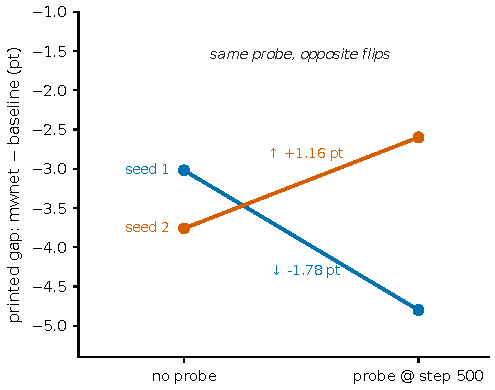
\includegraphics[width=3.3in]{figs/app_flip.pdf}%
}{%
  \fbox{\parbox[c][2.97cm][c]{0.55\textwidth}{\centering
    Placeholder for \texttt{figs/app\_flip.pdf}.}}%
}
\caption{The probe moves a printed method-versus-baseline comparison in
opposite directions on two seeds (Meta-Weight-Net official code). With a
probe at step 500, the printed gap moves from $-3.02$ to $-4.80$ points on
seed 1 (shift $-1.78$) and from $-3.76$ to $-2.60$ on seed 2 (shift
$+1.16$). Both movements are far above the family's accuracy-exact repeat
floor (Table~\ref{tab:floors}). These bidirectional displacements illustrate
the mechanism; Proposition~\ref{prop:pairing} does not predict a sign or a
zero mean across seeds.}
\label{fig:app-flip}
\end{figure}

% Supplementary figure: realistic-eval harvest (moved from main text for space).
\begin{figure}[t]
\centering
\IfFileExists{figs/fig_realeval.pdf}{%
  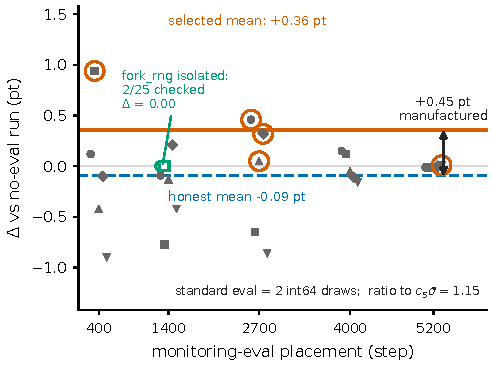
\includegraphics[width=3.3in]{figs/fig_realeval.pdf}%
}{%
  \fbox{\parbox[c][2.4cm][c]{0.55\textwidth}{\centering
    Placeholder for \texttt{figs/fig\_realeval.pdf}.}}%
}
\caption{The harvest reproduced by an \emph{unmodified} standard monitoring
evaluation, at a believable protocol (Meta-Weight-Net official code, full
$45$k train, $12$ epochs). A shuffled monitoring \texttt{DataLoader}'s two
$64$-bit seed draws desynchronize the pair; per-seed selection over five
placements manufactures $+0.45$ points (tracking $c_5\bar\sigma$, ratio
$1.15$), while the same evaluation inside \texttt{fork\_rng} is bitwise
inert in the directly checked model/meta-network hash pairs (2 of 25 cells).
This is scoped weight evidence, not a state-level check of all placements.
The full $120$-epoch campaign adds a same-codebase mechanism witness and
three directly checked repaired pairs; its Gaussian agreement remains a
small-sample, same-sample calibration.}
\label{fig:app-realeval}
\end{figure}

% Supplementary figure: guard-vs-LAWA payout bars.
\begin{figure}[t]
\centering
\IfFileExists{figs/app_payout_bars.pdf}{%
  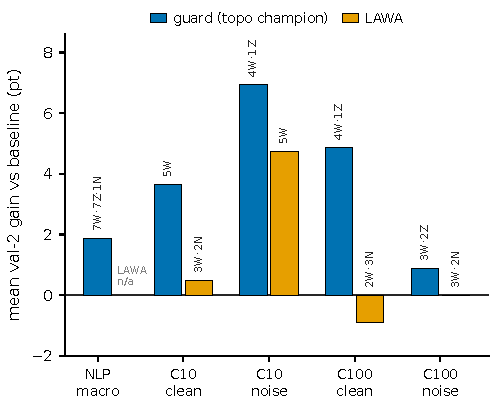
\includegraphics[width=3.3in]{figs/app_payout_bars.pdf}%
}{%
  \fbox{\parbox[c][2.97cm][c]{0.55\textwidth}{\centering
    Placeholder for \texttt{figs/app\_payout\_bars.pdf}.}}%
}
\caption{Guard payout versus LAWA across the five under-tuned cells, as
mean holdout gain over the paired baseline: guard $+1.88$ (NLP macro),
$+3.64$/$+6.95$ (CIFAR-10 clean/noise), $+4.86$/$+0.87$ (CIFAR-100
clean/noise); LAWA $+0.48$, $+4.73$, $-0.89$, $-0.00$ (not run on NLP).
Above each bar: per-unit win/zero/negative counts (15 task--seed cells for
NLP, 5 seeds per vision cell), where a zero is an \emph{exact} $0.00$
delta, not by itself a state-level certificate. The guard has one realized
loss ($-3.12$, RTE seed 1); LAWA is negative in $2$--$3$ units in three of
the four vision cells. These observed payouts do not bound the guard's
downside; the conditional no-op implication applies only under its premises.}
\label{fig:app-payout-bars}
\end{figure}

% Supplementary figure: guard vs always-EMA symmetry.
\begin{figure}[t]
\centering
\IfFileExists{figs/app_symmetry.pdf}{%
  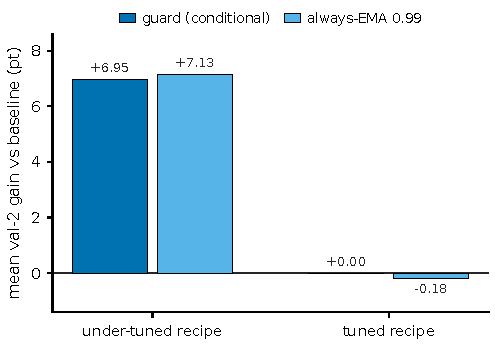
\includegraphics[width=3.3in]{figs/app_symmetry.pdf}%
}{%
  \fbox{\parbox[c][2.97cm][c]{0.55\textwidth}{\centering
    Placeholder for \texttt{figs/app\_symmetry.pdf}.}}%
}
\caption{The conditional guard against an unconditional always-EMA policy
(CIFAR-10, 30\% noise, deterministic, 5 seeds), as mean holdout gain over
the paired baseline. Under-tuned recipe: guard $+6.95$ versus always-EMA
$+7.13$; tuned recipe: guard exactly $0.00$ (all champions raw, metric-level
zeros) versus always-EMA $-0.18$. The $0.18$ points of upside conceded
where EMA helps accompanies an observed zero where it hurts; these metrics
alone do not establish a state-level certificate.}
\label{fig:app-symmetry}
\end{figure}

% Supplementary figure: per-cell NLP guard payout strip.
\begin{figure}[t]
\centering
\IfFileExists{figs/app_nlp_strip.pdf}{%
  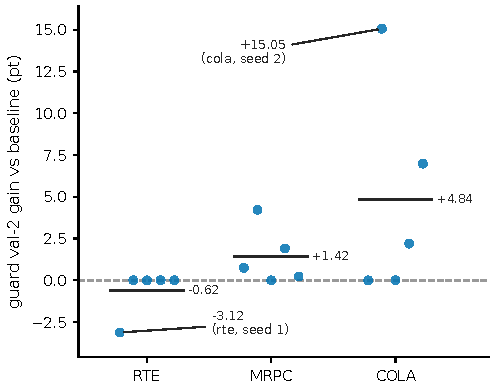
\includegraphics[width=3.3in]{figs/app_nlp_strip.pdf}%
}{%
  \fbox{\parbox[c][2.97cm][c]{0.55\textwidth}{\centering
    Placeholder for \texttt{figs/app\_nlp\_strip.pdf}.}}%
}
\caption{Per-cell guard payout on the under-tuned NLP campaign
(deterministic; 3 tasks $\times$ 5 seeds; champion from the selection log
versus the paired baseline's final holdout metric). Task means $-0.62$
(RTE), $+1.42$ (MRPC), $+4.84$ (CoLA); seven cells are exact zeros
(champion raw or holdout tie), and the extremes are the single realized
selection loss $-3.12$ (RTE seed 1) and the largest rescue $+15.05$ (CoLA
seed 2). The $-3.12$ cell is the observed loss reported rather than
averaged away.}
\label{fig:app-nlp-strip}
\end{figure}

% Supplementary figure: CoLA seed-2 case study.
\begin{figure}[t]
\centering
\IfFileExists{figs/app_cola_case.pdf}{%
  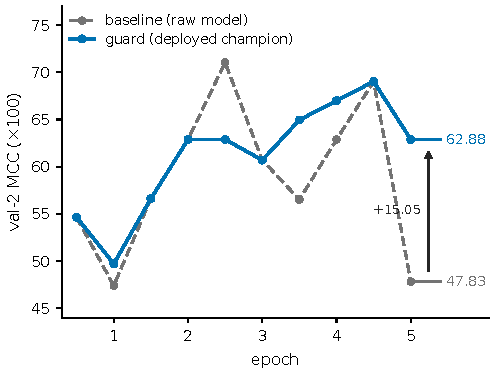
\includegraphics[width=3.3in]{figs/app_cola_case.pdf}%
}{%
  \fbox{\parbox[c][2.97cm][c]{0.55\textwidth}{\centering
    Placeholder for \texttt{figs/app\_cola\_case.pdf}.}}%
}
\caption{The CoLA seed-2 rescue behind the campaign's $+15.05$ cell
(deterministic pairing, same seed). The baseline's raw model collapses on
the final half-epoch (holdout MCC $\times 100$: $47.83$), while the
guard's deployed champion (EMA $0.999$, engaged by the epoch-1 fallback)
ends at $62.88$. The guard converts trajectory instability the baseline
merely suffers into a selection among stable candidates, which is what the
CoLA column of Figure~\ref{fig:app-nlp-strip} is made of.}
\label{fig:app-cola-case}
\end{figure}

\subsection{Where divergence starts: the traced MW-Net witness}
\label{sec:divergence-onset}

A dense causal trace on the Meta-Weight-Net rig localizes the onset of
divergence exactly (five frozen seeds; arms \code{base}, \code{shared\_eval},
\code{isolated\_eval}; all six preregistered gates pass: capture and trace
conservation, isolated restoration, single probe firing, repeat floor, and
two-draw replay), with one shuffled monitoring evaluation firing at step
$1400$ of $5400$. Figure~\ref{fig:divergence-onset} reads the resulting
layer-by-checkpoint relative-L2 grid cell by cell; what it establishes is that
divergence begins at a single identified draw (the meta-batch index draw
immediately after the probe, in all five seeds) and appears across the
whole network at once rather than creeping in through a slower channel, and
that restoring the stream cursors removes it bitwise.

% Divergence-onset heatmap (full-width, 7.0 x 4.6 in).
\begin{figure*}[t]
\centering
\IfFileExists{figs/fig_divergence_heatmap.pdf}{%
  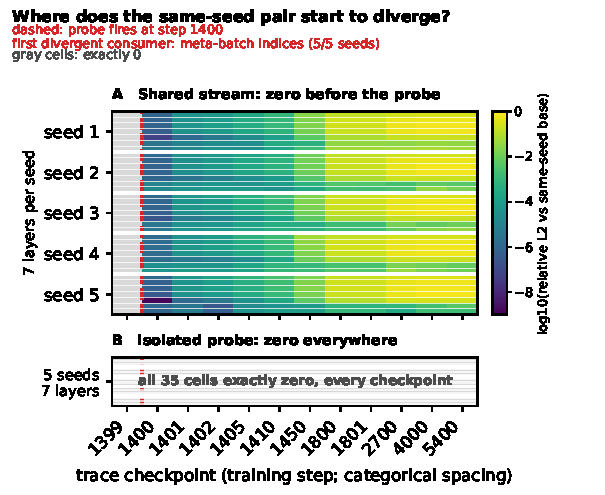
\includegraphics[width=\textwidth]{figs/fig_divergence_heatmap.pdf}%
}{%
  \fbox{\parbox[c][2.97cm][c]{0.9\textwidth}{\centering
    Placeholder for \texttt{figs/fig\_divergence\_heatmap.pdf}.}}%
}
\caption{Where the same-seed pair starts to diverge (MW-Net causal trace,
five seeds). Top: in the shared-stream arm, relative L2 against the
same-seed base is exactly zero (gray) for every layer and seed at the
pre-probe checkpoint and nonzero from the probe step ($1400$) onward; the
first divergent training-visible consumer is the meta-batch index draw in
all five seeds. Bottom: the isolated arm (the probe wrapped in a fork
with full RNG-state restoration) is exactly zero everywhere through step
$5400$. Within each seed block, rows are the frozen layer order (stem,
stages 1--3, head, then the meta-network's two layers); checkpoints are
unevenly spaced and drawn categorically. Layer-wise magnitude localizes
propagation without assigning causal responsibility for any final metric.}
\label{fig:divergence-onset}
\end{figure*}

% REMOVED: the CaffeNet sparse-RNG-trace subsection and its full-page archival
% figure. It was a preregistered eight-seed robustness confirmation on a
% classical CNN, and it replicated what Appendix D.4's MW-Net trace already
% shows: divergence begins at the first post-probe consumer, and the isolated
% arm stays byte-identical. Its distinct contribution was architectural
% breadth (a pre-ResNet topology), which no claim in the paper rests on. The
% run, its frozen artifacts, and figs/make_fig_caffenet_sparse_trace.py all
% remain in the repository. Nothing in the body or the appendix referenced
% \label{sec:caffenet} or \label{fig:caffenet} except this block itself.

\subsection{Independent nanoGPT prediction and supplemental diagnostics}
\label{sec:nanogpt-supplement}
The model is a tinyShakespeare nanoGPT with six layers, six heads and
embedding width 384, batch size 64, block length 256 and dropout 0.2.
The endpoint score averages eight fixed validation batches drawn with seed
20260908. Execution uses deterministic FP32 with TF32 disabled, math SDPA,
non-fused AdamW and no compilation. State checks cover weights/buffers,
optimizer, scaler, prefetched batches, update count, learning rate, module
modes, gradients and Python/NumPy/CPU/CUDA RNG at sparse checkpoints and the
endpoint, not every update.
The new campaign uses 16 calibration seeds (860901--860916) and 16
held-out seeds (860917--860932), five fixed placements and 2,000 updates.
There are 704 main runs: 32 seeds with 11 paths each (baseline, five shared
and five isolated), each run twice. Adding 22 runs for the separate pilot
seed 860899 gives 726 raw records; the pilot is excluded from analysis. Reconstructing
$D_{sj}=L_{s,\rm baseline}-L_{sj,\rm shared}$ from the raw fixed-panel
losses exactly reproduces both $16\times5$ analysis grids. Neither repeat
runs nor placement cells are treated as independent seeds.

The frozen primary prediction is $c_5\bar s/c_4(5)=0.00388406$, with
$c_5=1.16296447$, $c_4(5)=0.93998560$ and calibration mean sample SD
$\bar s=0.00313936$. Its observed-minus-predicted discrepancy is
$-0.00045346$ (approximate 95\% interval
$[-0.00134285,0.00043370]$). The \emph{prespecified uncorrected
sensitivity}, $c_5\bar s=0.00365096$, has prediction interval
$[0.00307846,0.00422724]$; relative to observed mean harvest $0.00343060$,
the discrepancy is $-0.00022036$ ($-6.04\%$), with interval
$[-0.00108275,0.00064263]$. This sensitivity does not replace the primary.
Both use 20,000 approximate percentile bootstrap draws (RNG seed
2026090801), independently resampling whole calibration and held-out seed
vectors, generating calibration indices first. The intervals do not
establish equivalence or identify a Gaussian residual law.

\paragraph{Exploratory reported-score decomposition.}
The following diagnostics were added after readout, unlike the sensitivity
above. Calibration selected maximum, unselected placement mean and harvest
are respectively $0.00462571$, $0.00034492$ and $0.00428079$, with
approximate 95\% intervals $[0.00254966,0.00678532]$,
$[-0.00133125,0.00201870]$ and $[0.00354967,0.00502692]$.
On held-out seeds they are $0.00324976$, $-0.00018085$ and $0.00343060$,
with intervals $[0.00149894,0.00490740]$,
$[-0.00165377,0.00128459]$ and $[0.00279334,0.00407564]$.
The selected fixed-panel mean's exploratory interval lies above zero.
Selection and scoring use the same panel, so this is not an independent
test improvement, and $H$ is not identified as pure reporting optimism.
The separate E1 validation-to-test bridge remains inconclusive.

\paragraph{Exploratory placement and influence diagnostics.}
In placement order $200,500,900,1300,1700$, calibration column means
(in $10^{-3}$ loss units) are
$(2.644,0.755,-1.054,-0.391,-0.230)$ and held-out means are
$(-0.059,-0.371,0.350,-0.355,-0.469)$.
Corresponding sample variances (in $10^{-5}$ squared loss units) are
$(4.274,2.526,1.028,1.092,1.125)$ and
$(1.980,2.383,1.588,1.255,1.318)$.
Raw off-diagonal covariance ranges are
$[5.241,23.483]\times10^{-6}$ and $[3.304,11.264]\times10^{-6}$;
correlations range $[0.382,0.881]$ and $[0.210,0.876]$.
These raw dependencies can include a common seed component and do not
by themselves reject conditionally iid residuals. Subtracting each seed's
placement mean gives contrast covariance ranges
$[-6.985,4.606]\times10^{-6}$ and $[-5.031,3.462]\times10^{-6}$,
and correlation ranges $[-0.694,0.791]$ and $[-0.690,0.684]$.
Centering mechanically imposes a sum-zero constraint; negative contrast
correlations are not an iid rejection either. These small-sample descriptive
diagnostics neither certify equal placement means/variances nor constitute
a formal Gaussian test; full matrices are released in
\code{revision\_results/nanogpt\_final/supplementary.json}.

Leaving out each calibration seed in turn gives corrected predictions
$[0.00372860,0.00400198]$. Leaving out each held-out seed, keeping the
full frozen prediction fixed, gives observed means
$[0.00329137,0.00355852]$ and discrepancies
$[-0.00059269,-0.00032554]$. These are influence ranges, not uncertainty
intervals or reasons to exclude seeds; all seeds remain in the primary.

\begin{figure}[t]
\centering
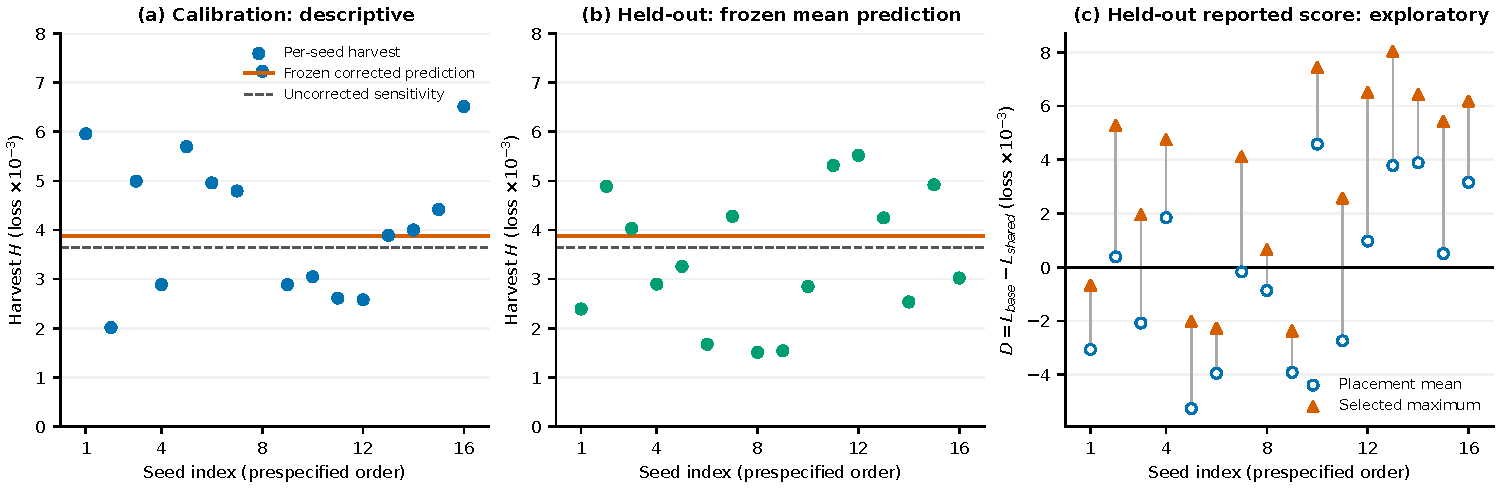
\includegraphics[width=\linewidth]{figs/nanogpt_per_seed.pdf}
\caption{Independent nanoGPT campaign, in prespecified seed order.
Left: descriptive calibration harvest. Middle: held-out harvest with the
frozen corrected prediction and prespecified uncorrected sensitivity;
horizontal lines predict a mean, not individual seeds. Right: exploratory
held-out selected maximum and placement mean on the same fixed validation
panel; connecting segments equal harvest. Repeats are not extra seeds.
The figure does not demonstrate independent-test transfer.}
\label{fig:nanogpt-per-seed}
\end{figure}

\subsection{Reproducibility and data availability}
\label{sec:availability}

The public repository
\url{https://github.com/dumingyu2004/silent-unpairing-tmlr2026} is the artifact
verified during review, with every later change listed in its
\code{RELEASE\_CHANGES.md}. It contains the raw results and analysis code
used for the reported harvest, E1 and verification summaries, together with
available run configurations, seeds, repeat records, exact upstream code
versions and source citations. It includes all 726 individual records from
the new nanoGPT campaign, its experiment and analysis scripts, frozen
prediction, and per-seed checks. Reanalysis from a fresh clone
reproduces the reported numerical results. Its README and file manifest
state what is included; this is an analysis-reproduction package, not a
claim that every historical training run can be repeated from it.

The repository also includes the two recovered historical MW-Net moneyshot
runners, source-backed explanatory repair diffs, and fifteen original
MW-Net endpoint files: baseline, repeat and isolated-probe model/meta-network
states for five seeds. Their stored tensor bytes agree within each seed;
these files do not contain complete optimizer, RNG or cursor state.
The diffs are revision-generated explanations against documented source
bases, not a recovered complete original repair-patch series.
A separate local trace companion retains seventeen original MW-Net tensor
archives for the five baseline/shared/isolated triplets and two baseline
repeats, checked against their retained run records. These seventeen NPZ
archives are not included in the public repository.

For E1, twenty split/noise input files are supplied as explicitly labelled
reconstructions from the retained source, seeds and configuration records.
The original runner generated these arrays in memory and exported only
configuration and results; it did not separately save them. The reconstruction
is checked against the source recipe, not against an unavailable original
array file. Clean dataset labels are external inputs to the supplied corruption
recipe. The repository therefore supports reanalysis and inspection of the
specified inputs and repairs without claiming every original checkpoint or
complete historical retraining coverage.

Historical writing and editing records reproduce the retained E1 runner and
protocol text exactly after newline normalization. The last content-changing
protocol edit is recorded at 10 July 2026, 14:56:39 UTC (11 July locally),
about 51 hours before the recorded campaign launch at 12 July 2026,
17:39:29 UTC. The repository includes a redacted chronology and verification
record in \code{docs/E1\_PROVENANCE.md} and
\code{revision\_results/e1\_provenance.json}.
For the new nanoGPT campaign, local controller records place the prediction
freeze at 8 September 2026, 18:55:00 UTC, before launching the held-out runs.
The available protocol and timing records are included with their provenance.
These are author-maintained pre-launch records, not independent external
registration; the chronology is based on recorded events rather than
copied-file dates.

\subsection{Extended monitoring and full-protocol harvest witnesses}
\label{sec:extended-harvest}

The harvest also does not need an inserted probe. Replacing the semantically
inert permutation draw with an \emph{unmodified} standard monitoring
evaluation (switch the model to evaluation mode, iterate a shuffled
validation loader for a few batches, switch back) reproduces the mechanism
at a believable protocol (Meta-Weight-Net official code, the full
$45{,}000$-image training set, $12$ epochs on the real three-phase schedule,
held-out test). The shuffled loader draws
exactly \emph{two} $64$-bit integers from the global stream training consumes,
its loader's base seed and its sampler's seed, with nothing inserted, and that
alone desynchronizes the pair: across $5$ seeds $\times\,5$ placements, per-seed
selection manufactures $+0.45$ points over the honest mean at ratio $1.15$ to
$c_5\bar\sigma$. The two directly checked isolated comparisons (two seeds,
placement 1400) match the never-evaluated baseline in final model and
meta-network parameters and buffers, with test-accuracy deltas exactly
$0.00$ (Figure~\ref{fig:app-realeval}). The remaining 23 repaired comparisons
were not directly verified; these two endpoints do not establish zero
selection gain across the placement grid. Together with
the state-purity inspection and controlled intervention, these repaired
comparisons support the stream-consumption explanation. Endpoint identity
alone cannot rule out transient changes that later reconverge. The effect is small at this
protocol and its size is not the claim: two integers drawn by a routine
validation loop suffice to manufacture a selectable, extreme-value-sized gain,
and the isolation wrapper restores endpoint equality in the two checked pairs.

The full official protocol closes the loop. At $120$ epochs ($58{,}800$
steps; repeat floor SHA-exact across all three seeds, model and
meta-network alike), the same rig sustains every layer: all twelve
placement$\times$seed pairs desynchronize bitwise, a single inert
permutation draw moves the printed method-versus-baseline gap by up
to $0.32$ points on the paper's best-accuracy metric ($0.56$ on final),
and per-seed best-of-four selection manufactures $+0.16$ points over the
honest mean,
with $c_4\bar\sigma = 0.16$ at ratio $1.0075$ using exact quadrature.
These are only three seeds; best and final are endpoints of the same runs,
not independent replications. The full plug-in simulations in Appendix~C do not
discriminate Gaussian from $t_3$ residuals. The same draw
inside a forked RNG state restores bitwise identity with the never-probed
baseline wherever we checked it (three of the twelve arms, verified by
model/meta-network SHA-256). Those three checked repaired deltas are zero;
we do not infer an all-placement bitwise check. Magnitudes anneal
with the schedule, as in the BHN witness; the measured mechanism and scoped
repair persist, while the Gaussian calibration remains conditional.

\section{Environment Manifest}
\label{sec:env}

\begin{itemize}\itemsep2pt
\item Python 3.12; PyTorch \code{2.11.0+cu128}; \code{transformers}
5.12.1; \code{accelerate} 1.14.0; NumPy 2.4.4.
\item Hardware: unless stated otherwise, a single NVIDIA GeForce RTX 5080
produced the registered floors and paired numbers. E1 used a separate Linux
host with one NVIDIA RTX PRO 6000 Blackwell, driver 595.71, and the same
PyTorch \code{2.11.0+cu128} build; its repeat-floor gate was rerun there
before launch and passed at model and meta-network SHA-256 resolution.
\item The new nanoGPT calibration/held-out campaign used an NVIDIA RTX PRO
6000 Blackwell Workstation Edition with PyTorch \code{2.11.0+cu128};
its per-path repeat checks were performed on that stack, not inferred from
the default RTX 5080 rig.
\item Framework citations in Appendix~B are pinned to \code{transformers}
5.12.1 and \code{torch} 2.11.0; audited repositories are pinned by commit
SHA (Tables~\ref{tab:classic} and~\ref{tab:recent}).
\item \code{scripts/rng\_premise\_check.py}: 13/13 assertions pass on this
stack, exercising both the CPU and the CUDA device.
\item \textbf{Scope of bitwise claims.} A bitwise floor checks repeatability
of its recorded state on its tested execution path, not pairing with a
different arm. Hardware, driver, or library changes can change the bits;
repeat checks must therefore be rerun per materially distinct path and stack.
The protocol is portable, not a guarantee of cross-platform bit identity.
\end{itemize}

\section{Supplementary Monitor Figures}
\label{sec:monitorfigs}

% No introductory paragraph. This section is its three figures; the heading is
% the pointer and each caption stands alone, so a sentence saying "Figure 13a
% shows the saturation" directly above a figure captioned "the saturation" was
% pure restatement. It also forced a text line onto the float page, which kept
% LaTeX from packing the three figures together. Consequence, deliberate: these
% three labels carry no \ref, so an orphan-float check will report them --
% that is the design here, not a regression.

% Supplementary figure: detector transfer grid.
\begin{figure}[t]
\centering
\IfFileExists{figs/app_detector_grid.pdf}{%
  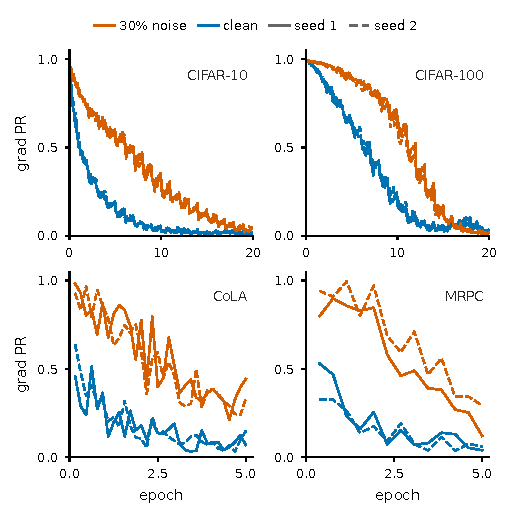
\includegraphics[width=3.3in]{figs/app_detector_grid.pdf}%
}{%
  \fbox{\parbox[c][2.97cm][c]{0.55\textwidth}{\centering
    Placeholder for \texttt{figs/app\_detector\_grid.pdf}.}}%
}
\caption{The participation-ratio detector transfers across datasets and
modalities: same-seed clean (blue) versus 30\%-noise (vermillion) runs,
two seeds each (solid/dashed), on CIFAR-10/100 (per-step monitor) and
CoLA/MRPC (per-40-step monitor). All 8/8 clean--noise pairs separate in
the early window; at the sample nearest epoch 1 the clean-versus-noise
gaps are $+0.27$ (CIFAR-10), $+0.52$ (CoLA), and $+0.68$ (MRPC), while
CIFAR-100's separation ($+0.04$ at epoch 1) opens over the following
epochs. Readings are same-dataset and seed-paired only: the scales differ
across datasets, the no-global-cutoff boundary.}
\label{fig:app-detector-grid}
\end{figure}

% Supplementary figure: trigger-statistic saturation.
\begin{figure}[t]
\centering
\IfFileExists{figs/app_saturation.pdf}{%
  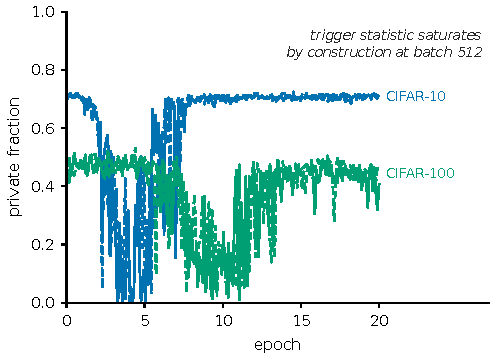
\includegraphics[width=3.3in]{figs/app_saturation.pdf}%
}{%
  \fbox{\parbox[c][2.97cm][c]{0.55\textwidth}{\centering
    Placeholder for \texttt{figs/app\_saturation.pdf}.}}%
}
\caption{The original private-fraction trigger statistic at batch 512
(deterministic clean campaigns, seeds 1--2): the statistic sits pinned at
its saturation plateau, run medians $0.70$ (CIFAR-10) and $0.44$
(CIFAR-100), apart from a transient mid-training dip window, and
carries no memorization signal at this batch size. This is the saturation
diagnosis (levels ${\approx}0.68$ and
${\approx}0.45$): the natural trigger never fires in the vision suite,
and the epoch-1 fallback engages the candidates instead.}
\label{fig:app-saturation}
\end{figure}

% Supplementary figure: late-window inversion.
\begin{figure}[t]
\centering
\IfFileExists{figs/app_latewindow.pdf}{%
  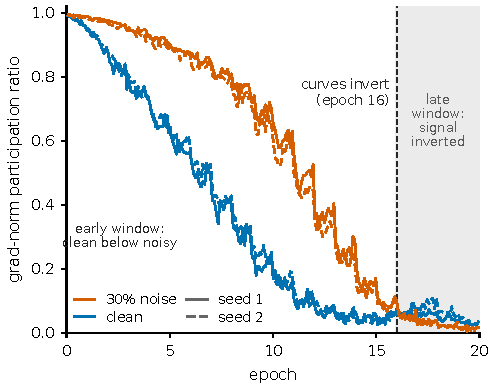
\includegraphics[width=3.3in]{figs/app_latewindow.pdf}%
}{%
  \fbox{\parbox[c][2.97cm][c]{0.55\textwidth}{\centering
    Placeholder for \texttt{figs/app\_latewindow.pdf}.}}%
}
\caption{The detector's operating window is early training (CIFAR-100
monitor study, full runs). The clean and 30\%-noise conditions are
separated from the first epoch (two-seed condition means $0.918$ vs.\
$0.978$), but as the training loss collapses the noisy curves fall
\emph{below} the clean ones (the condition means invert at epoch 16),
so late-window readings carry the signal with the wrong sign: readings
past the early epochs carry no information, the late-window
boundary.}
\label{fig:app-latewindow}
\end{figure}


\section{Extended context and discussion}
\label{sec:extended-context}

\subsection{Connections to prior work}

\paragraph{Reproducibility, nondeterminism, and causally valid comparison.}
Empirical work documents how small randomness sources amplify into large
run-level differences: a one-bit weight change drives a different final model
\citep{summers2021nondeterminism}, earlier perturbations diverge more (mirroring
our finding that a probe's \emph{timing} governs its effect)
\citep{altintas2025butterfly}, exact reproducibility is geometrically fragile
\citep{ly2025riddled}, and seeds and data order swing
results in reinforcement and active learning
\citep{henderson2018deep,ji2023randomness,patterson2024empirical}. A parallel line treats this
randomness as \emph{variance} to be budgeted across initializations, data
orders, and hyperparameters, then averaged over with more seeds
\citep{dodge2020finetuning,bouthillier2021accounting}. That line treats
performance as a distribution over seeds rather than a point estimate, and we
complement it from the other side: nothing here argues against reporting
distributions, but same-seed pairing is how two methods get compared without
paying for many seeds, and we show it can be invalidated from inside the
method. Desynchronization alone need not change the marginal mean effect;
its variance consequence depends on the coupling covariance. Selecting
favorable outcomes on the reported quantity adds directional optimism
(Proposition~\ref{prop:harvest}), which averaging already-selected outcomes
across seeds need not remove. The $+4.01$ demonstration uses this rule.
Unlike seed hacking, the
divergence is manufactured inside the method by its own probe and harvested by
its own selection step, with no researcher-side seed choice anywhere. It
inherits the statistics of model-selection over-fitting
\citep{cawley2010overfitting} but not its source: isolation removes the
probe-induced displacement at the checked resolution under the pairing premises.

The closest prior work sits in stochastic simulation, where misaligned
random-number realizations are a named problem: \citet{stout2008keeping}
prescribe synchronizing the numbers consumed by identical stochastic events;
\citet{klein2024noisefree} quantify the damage when that alignment fails,
reporting order-of-magnitude variance reductions once comparisons draw aligned
numbers; and \citet{buffalo2026realizing} formalize the causal failure (under a
stateful PRNG a path-altering intervention can shift draw indices on the aligned prefix,
voiding common-random-number counterfactuals) and repair it with counter-based
RNG. We build on this common-random-number alignment principle; our
contribution is its diagnosis in deep-learning evaluation, released-code
causal witnesses, and a connection to selection on the displaced quantity.
Nor is isolation tooling the gap:
splittable keys are a JAX design principle \citep{jax2018prng}, PyTorch ships a
fork-rng context manager \citep{pytorch_forkrng}, the mechanism surfaces in
issue trackers \citep{lightning2022rngissue} and RL tooling
\citep{matlab_rlevaluator}, and the common-random-number lineage is decades old
\citep{glasserman1992crn,pearce2022bayesian}. We do not claim a new general
principle of randomness or model selection. Section~\ref{sec:f2} connects
these established ideas through a checkable deep-learning mechanism and
separates reporting optimism from an unestablished held-out test improvement.

\paragraph{Reproducibility tooling and the harmlessness view.}
A systems literature makes bitwise-reproducible training practical and supplies
the operational half of our repair: record--replay and deterministic-execution
frameworks \citep{chen2022reproducible,heumos2023mlfcore} and verified
bit-identical pipelines \citep{shkolnikov2026bitidentical} show that an exact
repeat floor is attainable in practical systems. We use these tools rather
than compete with them: the contribution is not a determinism mechanism but the
observation that \emph{pairing validity}, not reproducibility of a single run,
is the property at stake. Closest in spirit,
\citet{zhuang2021randomness} characterize how tooling injects nondeterminism;
we localize a break in the paired comparison and demonstrate its directional
consequence when selection acts on the affected outcome.
\citet{jordan2024variance} argues that the between-run
test-set variance it measures is harmless and inevitable, which we do not dispute: pairing
exists precisely to see \emph{through} that variance, and our result is that
the instrument can fail, while selection on the reported quantity creates
optimism; observed uplift can also contain systematic placement effects.

\paragraph{Bilevel meta-learning and sample reweighting.}
Learning-to-reweight methods learn per-example weights through a virtual
optimizer step and a meta-objective on held-out data: L2RW
\citep{ren2018learning}, Meta-Weight-Net \citep{shu2019metaweightnet}, the
co-training lineage of Co-teaching \citep{han2018coteaching} and DivideMix
\citep{li2020dividemix}, recent entries BHN \citep{yu2023bhn} and RENT
\citep{bae2024rent}, and a three-phase reweighting theory
\citep{zhang2025revisiting}. This is the audit's home neighborhood. A
second\diagtwoscope{}
diagnosis speaks to this family: the canonical lr-scaled
virtual step emits an exactly $\eta$-scaled meta-signal, which can be dominated
where an $\eta$-independent term of comparable or larger size competes for the
same weights, a magnitude ratio rather than an inevitability;
\diagtwopointer{}.

\paragraph{Weight averaging.}
Our guarded averaging endpoint illustrates the conditional no-op, rather
than claiming an accuracy advantage over SWA, model soups, trainable/early
averaging, LAWA, or adaptive averaging
\citep{izmailov2018averaging,wortsman2022soups,li2023twa,sanyal2024early,
kaddour2022lawa,demir2024aswa,melis2022twotailed,wang2025sewa,ajroldi2025when}.
The auxiliary comparisons are retained in the appendix.

\subsection{Practical implications and detailed scope}


\paragraph{A norm that would close the gap.}
Probe consumption of a stream later used by training can break trajectory
alignment. Proposition~\ref{prop:pairing} gives a sufficient preservation
condition and localizes update-relevant divergence; mere stream sharing
is not enough. The Trainer's
sequential-sampler/no-grad evaluation is stream-disjoint from training in the tested configuration
(Table~\ref{tab:hf}), and frameworks that
isolate probe RNG (Lightning's isolate-rng utility
\citep{falcon2019lightning}, fairseq's re-keying \citep{ott2019fairseq}, JAX's
splittable keys \citep{jax2018prng}) ship the primitives that enforce
isolation, though whether a given program is isolated still depends on how it
assigns probe and training keys. Isolation is
often small as a code change, but it must be \emph{checked}, not assumed:
deterministic kernels and a per-path repeat/state audit add real runtime and
storage costs, and some platforms lack deterministic implementations. The
three practices of Section~\ref{sec:repair} make the check mechanical. A
venue-level norm of repeat-floor reporting would make this artifact class
checkable, not cost-free.

\paragraph{Selection optimism.}
The general selection decomposition separates reporting optimism from
systematic placement effects without independence assumptions. Selecting
the best of $m$ candidates has expected uplift $c_m\sigma$ only under the
stated iid-Gaussian benchmark (Proposition~\ref{prop:harvest}); correlated,
heteroscedastic, or offset placements need not obey that scale: classical
selection bias \citep{cawley2010overfitting}, fed here by divergence the
instrument manufactures. Observed max-minus-mean uplift is not identified
as pure optimism or held-out gain: it also contains placement effects.
The no-op corollary is an application of the pairing condition, not a
claim that selecting or averaging candidates improves accuracy. Its
auxiliary candidate-selection analyses remain separate from the core
evaluation diagnosis.

\paragraph{Distinct safeguards and remaining limits.}
State-pure isolation preserves coupling under the proposition's premises.
Independent-seed comparisons have no exact coupling to lose, but can still
suffer selection optimism. Omitting selection removes this source of
directional optimism, not the displacement or its possible variance effect.
A large true effect does not restore pairing. Every measurement
here is single-process, and we have not tested the artifact under distributed
training of any topology, which we leave as future work. Our method
claims are at academic scale (ResNet-18, RoBERTa-base; nanoGPT enters only the
artifact analysis) and cover label noise rather than distribution drift, and in
tuned regimes the reported guard gain is metric-zero; historical evidence
does not establish a state-level certificate for every cell. The artifact's \emph{dynamic}
evidence spans CIFAR-10 convnets, two GLUE tasks on RoBERTa-base, and nanoGPT
at 200 iterations and a separate 2,000-update calibration/held-out campaign,
with nothing claimed at ImageNet or production-LLM scale. The latter freezes
its scale on 16 calibration seeds and checks a mean on 16 held-out seeds;
it does not validate a universal Gaussian model, per-run prediction, or
independent-test transfer (Section~\ref{sec:harvest}). The core eleven-of-eleven audit is double-read,
and seven of its entries and the entire field-wide wave are static findings,
labeled as such, with pinned commits released for re-execution.


\end{document}
